% Template for PLoS
% Version 3.1 February 2015
%
% To compile to pdf, run:
% latex plos.template
% bibtex plos.template
% latex plos.template
% latex plos.template
% dvipdf plos.template
%
% % % % % % % % % % % % % % % % % % % % % %
%
% -- IMPORTANT NOTE
%
% This template contains comments intended 
% to minimize problems and delays during our production 
% process. Please follow the template instructions
% whenever possible.
%
% % % % % % % % % % % % % % % % % % % % % % % 
%
% Once your paper is accepted for publication, 
% PLEASE REMOVE ALL TRACKED CHANGES in this file and leave only
% the final text of your manuscript.
%
% There are no restrictions on package use within the LaTeX files except that 
% no packages listed in the template may be deleted.
%
% Please do not include colors or graphics in the text.
%
% Please do not create a heading level below \subsection. For 3rd level headings, use \paragraph{}.
%
% % % % % % % % % % % % % % % % % % % % % % %
%
% -- FIGURES AND TABLES
%
% Please include tables/figure captions directly after the paragraph where they are first cited in the text.
%
% DO NOT INCLUDE GRAPHICS IN YOUR MANUSCRIPT
% - Figures should be uploaded separately from your manuscript file. 
% - Figures generated using LaTeX should be extracted and removed from the PDF before submission. 
% - Figures containing multiple panels/subfigures must be combined into one image file before submission.
% For figure citations, please use "Fig." instead of "Figure".
% See http://www.plosone.org/static/figureGuidelines for PLOS figure guidelines.
%
% Tables should be cell-based and may not contain:
% - tabs/spacing/line breaks within cells to alter layout or alignment
% - vertically-merged cells (no tabular environments within tabular environments, do not use \multirow)
% - colors, shading, or graphic objects
% See http://www.plosone.org/static/figureGuidelines#tables for table guidelines.
%
% For tables that exceed the width of the text column, use the adjustwidth environment as illustrated in the example table in text below.
%
% % % % % % % % % % % % % % % % % % % % % % % %
%
% -- EQUATIONS, MATH SYMBOLS, SUBSCRIPTS, AND SUPERSCRIPTS
%
% IMPORTANT
% Below are a few tips to help format your equations and other special characters according to our specifications. For more tips to help reduce the possibility of formatting errors during conversion, please see our LaTeX guidelines at http://www.plosone.org/static/latexGuidelines
%
% Please be sure to include all portions of an equation in the math environment.
%
% Do not include text that is not math in the math environment. For example, CO2 will be CO\textsubscript{2}.
%
% Please add line breaks to long display equations when possible in order to fit size of the column. 
%
% For inline equations, please do not include punctuation (commas, etc) within the math environment unless this is part of the equation.
%
% % % % % % % % % % % % % % % % % % % % % % % % 
%
% Please contact latex@plos.org with any questions.
%
% % % % % % % % % % % % % % % % % % % % % % % %

\documentclass[10pt,letterpaper]{article}
\usepackage[top=0.85in,left=2.75in,footskip=0.75in]{geometry}

% Use adjustwidth environment to exceed column width (see example table in text)
\usepackage{changepage}
\usepackage{tabularx}
% Use Unicode characters when possible
\usepackage[utf8]{inputenc}

% textcomp package and marvosym package for additional characters
\usepackage{textcomp,marvosym}

% fixltx2e package for \textsubscript
\usepackage{fixltx2e}

% amsmath and amssymb packages, useful for mathematical formulas and symbols
\usepackage{amsmath,amssymb}

% cite package, to clean up citations in the main text. Do not remove.
\usepackage{cite}

% Use nameref to cite supporting information files (see Supporting Information section for more info)
\usepackage{nameref,hyperref}

% line numbers
%\usepackage[right]{lineno}

% ligatures disabled
\usepackage{microtype}
\DisableLigatures[f]{encoding = *, family = * }

% rotating package for sideways tables
\usepackage{rotating}

\usepackage{color}

% Remove comment for double spacing
%\usepackage{setspace} 
%\doublespacing

% Text layout
\raggedright
\setlength{\parindent}{0.5cm}
\textwidth 5.25in 
\textheight 8.75in

% Bold the 'Figure #' in the caption and separate it from the title/caption with a period
% Captions will be left justified
\usepackage[aboveskip=1pt,labelfont=bf,labelsep=period,justification=raggedright,singlelinecheck=off]{caption}

% Use the PLoS provided BiBTeX style
\bibliographystyle{plos2015}

% Remove brackets from numbering in List of References
\makeatletter
\renewcommand{\@biblabel}[1]{\quad#1.}
\makeatother

% Leave date blank
\date{}

% Header and Footer with logo
\usepackage{lastpage,fancyhdr,graphicx}
\usepackage{epstopdf}
\pagestyle{myheadings}
\pagestyle{fancy}
\fancyhf{}
\lhead{
\includegraphics[width=2.0in]{PLOS-submission.eps}}
\rfoot{\thepage/\pageref{LastPage}}
\renewcommand{\footrule}{\hrule height 2pt \vspace{2mm}}
\fancyheadoffset[L]{2.25in}
\fancyfootoffset[L]{2.25in}
\lfoot{\sf PLOS}

%% Include all macros below

\newcommand{\lorem}{{\bf LOREM}}
\newcommand{\ipsum}{{\bf IPSUM}}

%% END MACROS SECTION


\begin{document}
\vspace*{0.35in}

% Title must be 250 characters or less.
% Please capitalize all terms in the title except conjunctions, prepositions, and articles.
\begin{flushleft}
{\Large
\textbf\newline{gr-MRI: A software package for magnetic resonance imaging using software defined radios}
}
\newline
% Insert author names, affiliations and corresponding author email (do not include titles, positions, or degrees).
\\
Christopher J. Hasselwander\textsuperscript{1,3,\Yinyang},
Zhipeng Cao\textsuperscript{1,3,\ddag},
William A. Grissom\textsuperscript{1,2,3,\Yinyang}
\\
\bigskip
\bf{1} Department of Biomedical Engineering, Vanderbilt University, Nashville, Tennessee, USA
\\
\bf{2} Department of Radiology and Radiological Sciences, Vanderbilt University, Nashville, Tennessee, USA
\\
\bf{3} Vanderbilt University Institute of Imaging Science, Nashville, Tennessee, USA
\\
\bigskip

\end{flushleft}
% Please keep the abstract below 300 words
\section*{Abstract}
{\bf Purpose:} To develop software that enables the rapid implementation of custom MRI spectrometers using commercially-available software defined radios (SDRs).\\[1em]

\noindent{\bf Methods:} The gr-MRI software package comprises a set of Python scripts, flowgraphs, and 
signal generation and recording blocks for GNU Radio, 
an open-source SDR software package that is widely used in communications research. 
gr-MRI Implements basic event sequencing functionality, 
and tools for system calibrations, multi-radio synchronization, and 
MR signal processing and image reconstruction. 
It includes four pulse sequences: 
a single-pulse sequence to record free induction signals, 
a gradient-recalled echo imaging sequence, a spin echo imaging sequence,
and a spin echo inversion recovery imaging sequence.

\par The gr-MRI sequences were used to perform phantom imaging scans with a 0.5 Tesla 
tabletop MRI scanner and two commercially-available SDRs.
One SDR was used for RF excitation and reception, and the other for gradient pulse generation. 
The total SDR hardware cost was approximately \$2000.
The frequency of radio desynchronization events and the frequency with which the software recovered from those events was also measured,
and
the SDR's ability to generate frequency-swept RF waveforms was 
validated and compared to the scanner's spectrometer.\\[1em]

\noindent{\bf Results:} Gradient echo 
and spin echo images geometrically matched those 
acquired using the scanner's spectrometer, with no unexpected distortions.
Inversion recovery images exhibited expected behavior as a function of inversion time.
Desynchronization events were more likely to occur at the very beginning of an imaging scan,
but were nearly eliminated if the user invokes the sequence for a short period before 
beginning data recording.
The SDR was able to produce a 500 kHz bandwidth frequency-swept pulse with high fidelity, 
while the scanner's spectrometer produced a waveform with large frequency spike errors. \\[1em]

\noindent{\bf Conclusion:} The developed gr-MRI software can be used to develop high-fidelity, 
low-cost custom MRI spectrometers 
using commercially-available SDRs. \\[1em]

% Note that timing and synchronization issues are dealt with

% Please keep the Author Summary between 150 and 200 words
% Use first person. PLOS ONE authors please skip this step. 
% Author Summary not valid for PLOS ONE submissions.   
%\section*{Author Summary}
%
%???

%\linenumbers

\section*{Introduction}
% The Introduction should say:
% - There is a reason to investigate alternative spectrometer architectures
% - Current alternative architectures are expensive (Medusa, TecMag, Kia, NI boards (Wright and Hashimoto)) or require considerable hardware development which requires hardware expertise
% - Software defined radios are simple, cheap hardware since they are essentially just RF sound cards that offload most processing to the CPU, and SDR spectrometers have been developed for NMR previously.
% - There are also a lot of commercial SDRs that could be used for MR and they are all supported by GNURadio, but there is no software to support that use. 
% - We have developed that software to do X, and we have validated it in experiments doing Y. 
% - This will enable researchers to develop custom MR spectrometer solutions using off-the-shelf hardware, without hardware expertise and with minimal software development, and without FPGA programming expertise
Modern commercial magnetic resonance imaging (MRI) and nuclear magnetic resonance (NMR) spectrometers are sophisticated devices with very high performance. 
However, many research and development applications in magnetic resonance require more configurable, portable, or scalable spectrometers at a lower cost than commercial offerings.
For example, spectrometers have been developed in-house to meet the unique needs of low-field MRI scanners \cite{jie:hbmr:2005,wright:2002},
deliver point-of-care relaxometry measurements \cite{peng:domp:2012},
hyperpolarize exogenous contrast agents \cite{parnell:dpns:2008},
increase the number of receive channels in parallel imaging \cite{bodurka:smmd:2004,tang:adrm:2012,stang:medusa:2012},
implement parallel transmission \cite{stang:medusa:2012,Toronto145,4915785},
and acquire signals in NMR field monitoring probes concurrently with imaging \cite{barmet:atrs:2009,sipila:2HTR:2011,sipila:dmrf:2009}. 
In particular, many recent systems have been designed around field programmable gate arrays (FPGAs) which perform sequencing and signal processing functions \cite{gengying:dnmr:2001,jie:hbmr:2005,takeda:ahif:2007,opencorenmr,tang:2011,peng:domp:2012,stang:medusa:2012}.
FPGAs are particularly well-suited for MR at Larmor frequencies of tens to hundreds of megahertz
since they can process multiple streams of transmitted and received data in parallel at high speeds.

\par While FPGAs are well-suited to application in high-frequency MR spectrometers, 
replicating current FPGA-based spectrometers is challenging for non-electronics experts
due to the steep learning curve involved in FPGA programming,
and since most are based on custom circuit designs that would be
difficult for non-experts to recreate.
At the same time, communications research has benefited in recent years from the development
of the open-source GNU Radio software (gnuradio.org), 
which enables non-hardware experts to build custom software radios that can be used with a wide range of low-cost 
software-defined radio (SDR) devices; at the time of writing, the GNU Radio website list ten compatible SDR vendors, many of which offer several  SDR models \cite{gnuradiovendors}. 
SDR's typically comprise analog-to-digital and digital-to-analog converters,
an FPGA for basic filtering and signal down- and up-conversion, 
and a USB interface. 
They can be thought of as PC sound cards that operate at RF frequencies, in that
they act as an interface between the digital computer and the analog world, 
while the PC handles most of the real-time digital signal manipulations. 
Depending on their feature set, 
commercial GNU Radio-compatible SDR's currently cost between a few hundred and a few thousand dollars and ship with FPGA software images,
so the user can focus on implementing the functionality of their radios on the PC side.
Software radios are built in the Python programming language (python.org) in GNU Radio, 
by connecting modular signal processing components together
into a flowgraph, the inputs and outputs of which are connected to the SDR via a driver interface. 

\par We describe an open-source software package that extends the functionality of GNU Radio to perform
MRI experiments. 
The package comprises a set of Python scripts and two C++-based GNU Radio flowgraph elements.
It implements system timing calibrations, center frequency and transmit power optimization, 
shaped RF and gradient pulses, image reconstruction, 
and three representative MR imaging sequences: spin echo, gradient echo, and inversion recovery.
It was used to operate a commercial 0.5 Tesla tabletop MRI scanner with a pair of commercially-available SDRs to generate 
all RF and gradient pulses and sample received signals.
Overall, the software will enable users to rapidly implement custom MRI spectrometers, 
without recreating or developing new hardware. 
Since it is built on top of the active GNU Radio project, 
the software will be compatible with a wide range of current and future SDR devices.

%
%
%, there is a lack of available software for SDR enabled MRI, which may be a significant barrier to researchers who wish to home-build scanners.
%
%\par In this work we describe a SDR enabled MRI software package called gr-MRI that we paired with the commercially-available Ettus Research USRP1.  The gr-MRI software package is offered as a free software package and aims to provide a cheap, flexible, and easy to use alternative to traditional MRI spectrometers.  The package is built on top of GNU Radio (version 3.7.5.1), an open source and actively developed SDR interfacing signal processing software.  The package includes three stock imaging sequences: a slice-selective spin echo, slice-selective gradient echo, and slice selective spin echo inversion recovery sequence, which were validated using a 0.5 Tesla Oxford Maran scanner (Resonance Instruments, Witney, UK) with a center frequency of roughly 21.3 MHz.  The resulting spin echo and gradient echo images shown have a slice thickness of 4mm, FOV of 20 mm on a 128 by 128 grid.  The spin echo inversion recovery sequence was validated via a $T_1$ mapping study.

\section*{Methods}

\subsection*{A basic single-pulse sequence in GNU Radio}
To illustrate how GNU Radio works and to motivate the architecture and features of the
gr-MRI package, 
Figure \ref{fig:singlepulse}a shows an implementation of the most basic NMR pulse sequence using GNU Radio alone, without the gr-MRI software package. 
The sequence comprises a single-pulse excitation with simultaneous reception of the free induction decay (FID) signal. 
Specifically, 
the figure shows a graphical representation of this sequence's flowgraph in 
GNU Radio Companion (a GUI-based flowgraph editor packaged with GNU Radio).
A GNU Radio flowgraph is made up of signal generation, signal processing, and input and output blocks,
which are connected by virtual wires that transmit baseband signals between them; 
wires conduct signals in one direction. 
In this flowgraph, the blocks that produce a block excitation pulse are outlined in box A.  
The pulse is generated by duplicating a square wave, inverting and delaying its copy, and multiplying the copy by itself. 
Then the real-valued block pulse signal is converted to a complex signal type (with zero imaginary
component) and passed into the USRP Sink block 
(box B), which interfaces via a driver to one or more transmit 
channels of a Universal Software Radio Peripheral SDR (USRP; Ettus Research, Santa Clara, CA, USA). 
The demodulated received signal comes back into the flowgraph via the USRP Source block (box C), 
which sends the amplitude of the signal to an oscilloscope block
for continuous display (box D). 
The flowgraph is free-running, and does not record data.
\textcolor{red}{Figure \ref{fig:singlepulse}b shows the oscilloscope window that appears when the flowgraph is executed, 
which displays the demodulated FID signal in real-time.}

\begin{figure}[!ht]
\begin{center}
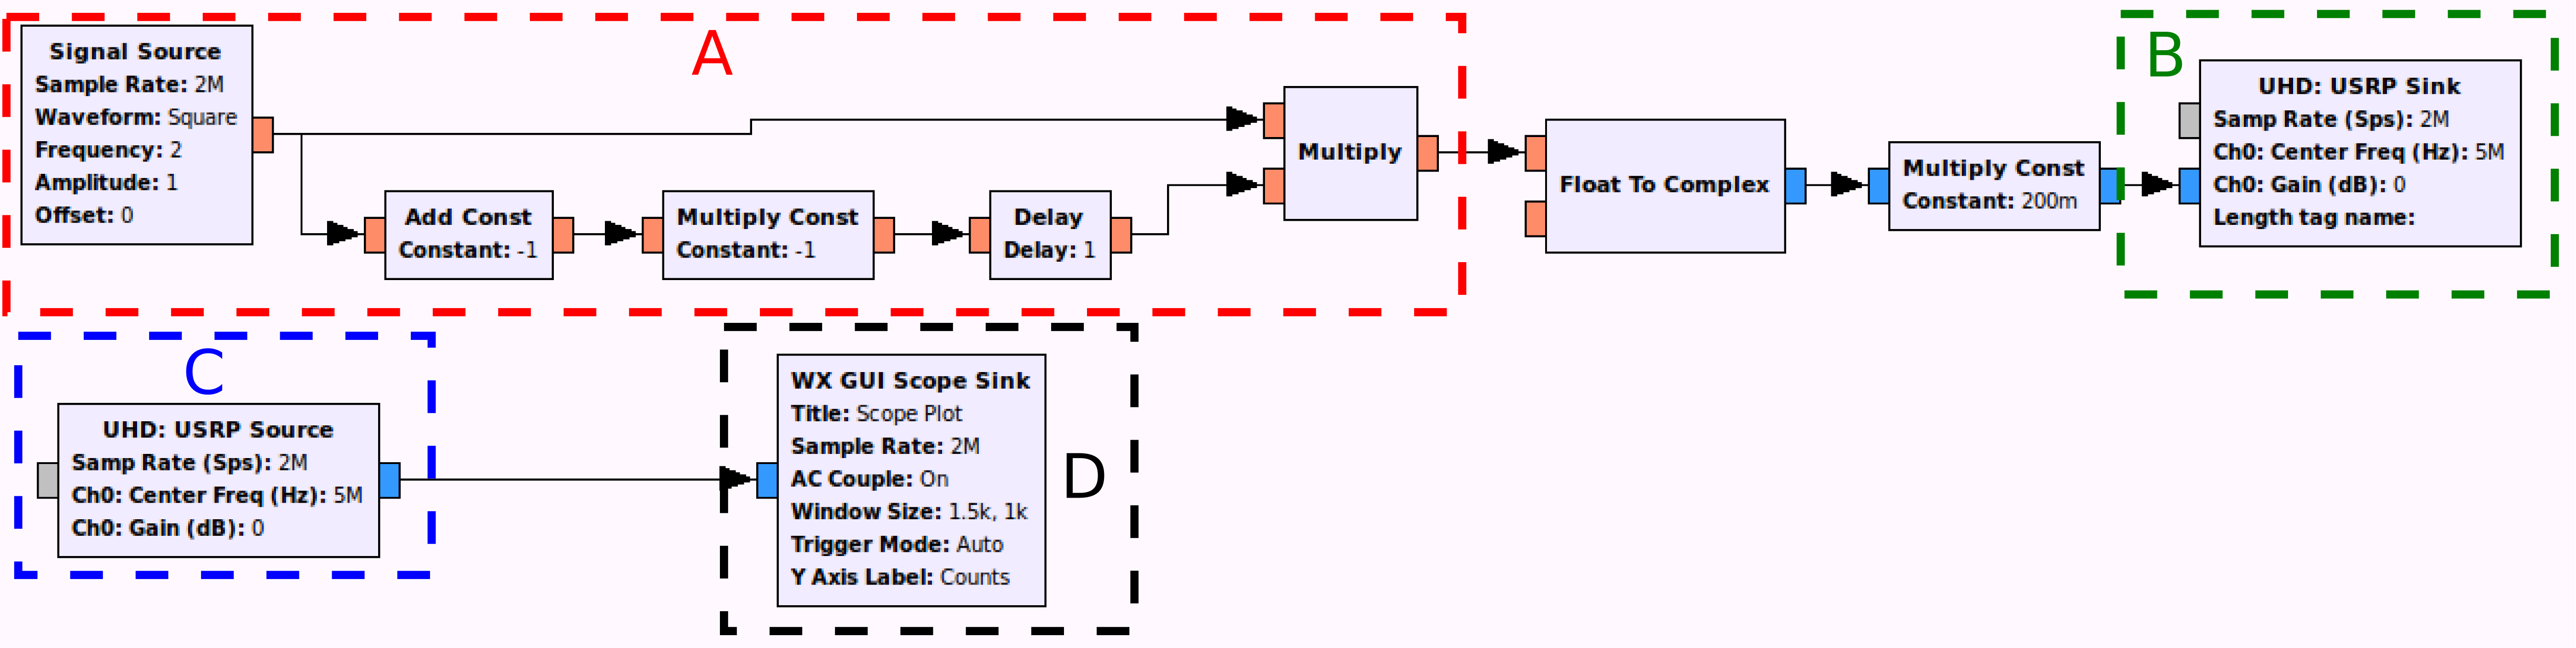
\includegraphics[width = \textwidth,trim=0 0 0 0,clip=false]{simple_tx_rx.png}
\caption{Basic single-pulse GNU Radio flowgraph without gr-MRI elements.  
The outlined boxes contain: 
A) The excitation pulse generation blocks, 
B) the USRP Sink block which sends the excitation pulse to the radio, 
C) the USRP Source block which receives baseband RF signals from the radio, 
and D) the oscilloscope block to continuously display the received signal.}
\label{fig:singlepulse}
\end{center}
\end{figure}

\par This example illustrates that GNU Radio flowgraphs run continuously and are not inherently sequenced
as is required for MR.
Furthermore, the precise timing of transmitted signals is subject to delays on the PC,
and the software lacks the ability to generate shaped waveforms such as sinc excitation pulses and gradient trapezoids,
as well as the ability to change pulse amplitudes and phases between repetitions.  
It also lacks the ability to selectively record received signals over specific time intervals. 
To address these needs, gr-MRI pulse sequences use master clock signals that trigger 
provided RF and gradient pulse generation and signal recording blocks.   
gr-MRI further provides tools to calibrate gradient strength, center frequency, and RF power,
and to synchronize sequence timing in order to compensate system
delays between RF and gradient pulse transmission and signal reception. 
These tools and features are described in the next sections.

\subsection*{Sequenced pulse generation and signal recording in gr-MRI}
gr-MRI Uses square wave signals with period equal to the sequence repetition time (TR) 
(or TR plus inversion time (TI) in an inversion recovery sequence, described further below) to trigger pulse sequence events.
To generate shaped RF and gradient pulses, 
gr-MRI provides a C++-based \textit{Triggered Vector Source} block, illustrated in Figure~\ref{fig:tvs}a. 
The block plays real- or complex-valued samples from a user-provided vector that is typically loaded when it is constructed but can also be changed during sequence execution.  
After its pulse has been played completely, 
a Triggered Vector Source plays zeros until it receives another trigger.
The settings (Figure~\ref{fig:tvs}b) allow the user to specify 
amplitude stepping for phase encode gradients and RF chopping, 
and how many times to repeat each step to accommodate averaging.
Received signals are recorded using the \textit{Gated Vector Sink} block, shown in Figure~\ref{fig:tvs}c, 
which writes a complex data stream from one input to an internal vector whenever its other input is high.  

\par To initiate a gr-MRI scan sequence, 
the user invokes that sequence's Python script from the IPython shell \cite{PER-GRA:2007}, which
creates the RF and gradient waveforms and loads
them into Triggered Vector Sources in a new sequence flowgraph.
The script then optionally launches the flowgraph into an interactive prescan period, 
during which the user can dynamically adjust sequence parameters such as timing and pulse amplitude settings from the command line,
and observe the effect on the received signal which is displayed in real time.
Finally the user invokes the full scan,
and the entire sequence is run while the script saves raw data into the Gated Vector Sink.
After the scan, the user can extract the data from the Gated Vector Sink into a k-space matrix,
and reconstruct an image using provided functions described below.

\begin{figure}[!ht]
\begin{center}
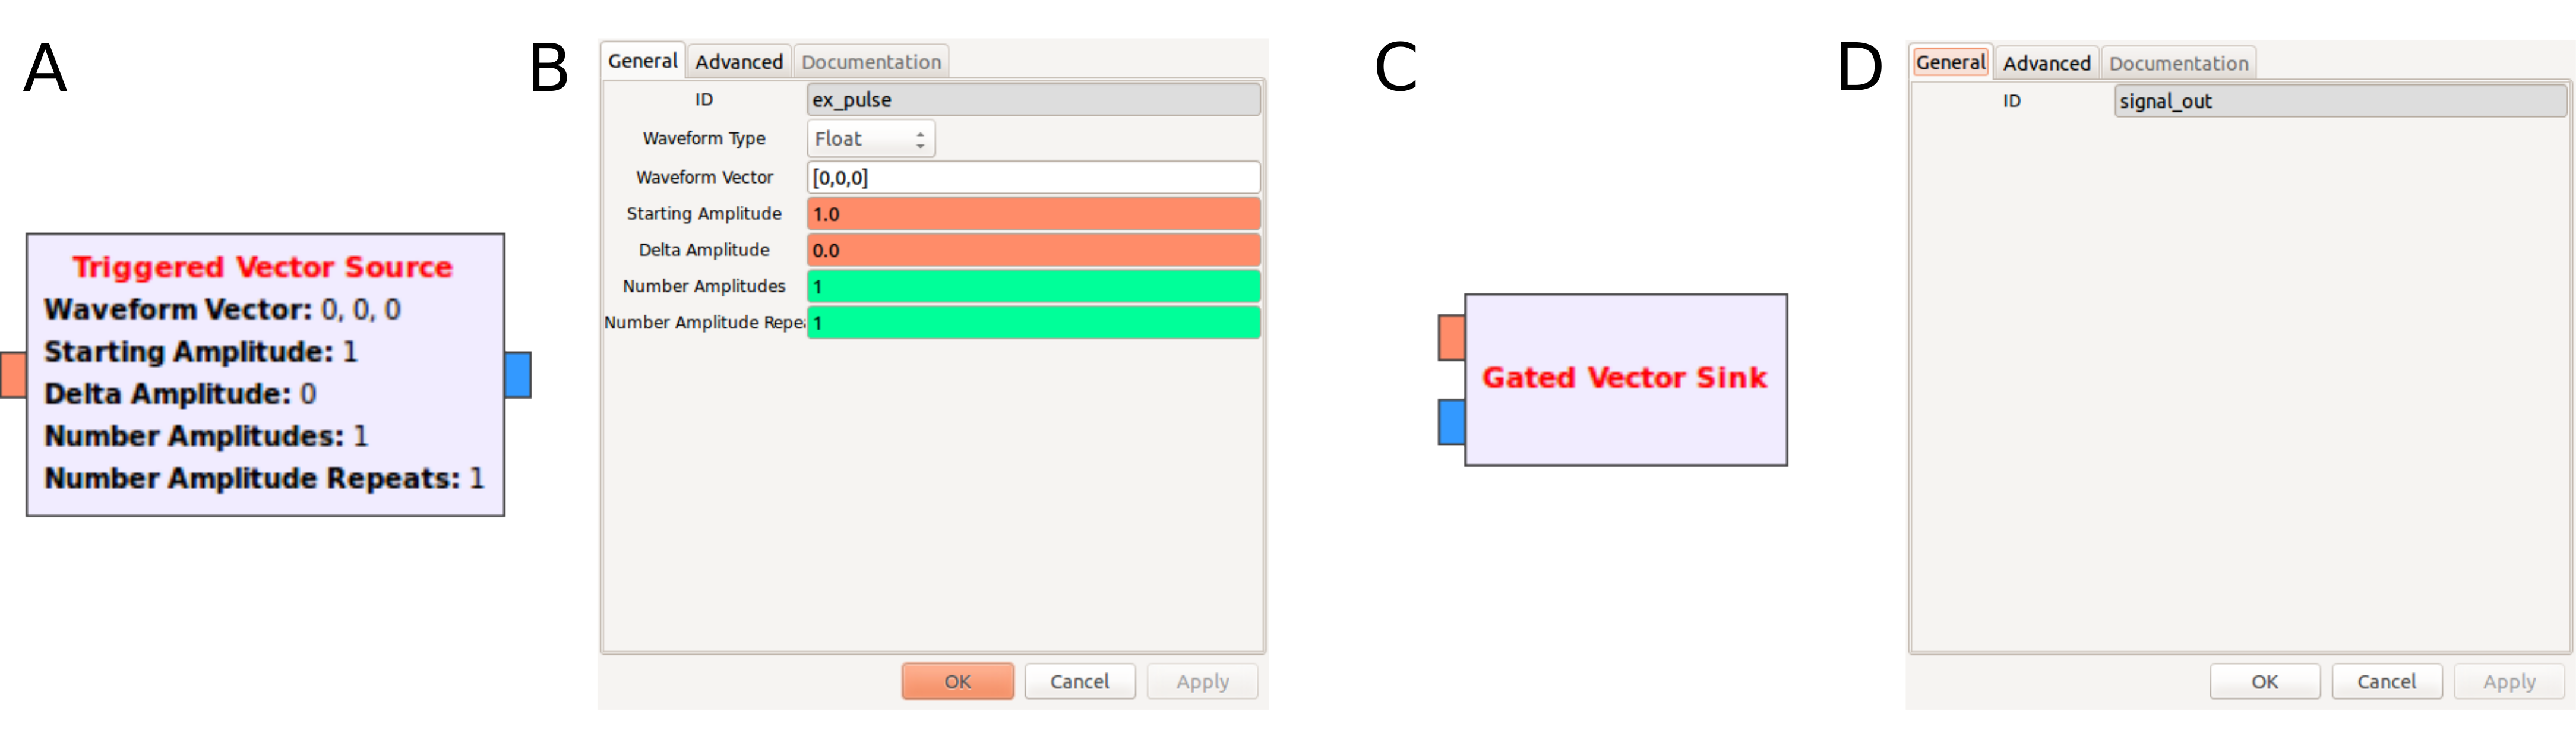
\includegraphics[width = \textwidth,trim=0 0 0 0,clip=false]{custom_blocks.png}
\caption{A) The Triggered Vector Source GNU Radio block.  
The orange box on the left is the block's input socket and the blue box on the left is its output socket. 
B) The Triggered Vector Source block's settings.  
C) The Gated Vector Sink GNU Radio block.  
The blue box on the left represents the complex data input socket, 
and the orange box represents the gate socket which controls data recording. 
D) The Gated Vector Sink block's settings.}
\label{fig:tvs}
\end{center}
\end{figure}

\subsection*{gr-MRI Pulse sequences}
\paragraph{Basic single-pulse: \texttt{FID.py}} Figures \ref{fig:txflow} and \ref{fig:rxflow} show a gr-MRI-enabled 
flowgraph that implements the same single-pulse sequence as in Figure \ref{fig:singlepulse}, 
but uses a Triggered Vector Source to generate arbitrary RF excitation pulses,
and a Gated Vector Sink to record data. 
Figure \ref{fig:txflow} shows the flowgraph's transmit section.  
The outlined box A contains the TR clock signal generator that produces a square wave with period equal to the TR.  
The output signal triggers two Triggered Vector Sources in outlined box B, 
which are each loaded with a waveform and settings defined in the 
Python script.
The top Triggered Vector Source produces a scalable block excitation pulse which is sent to the RF power amplifier, 
and the bottom one generates a longer block pulse that defines the signal recording interval.  
The latter signal is transmitted from the SDR and fed back into one of the SDR's receive channels to trigger the Gated Vector Sink in Figure \ref{fig:rxflow} for signal recording.  
This loopback mechanism is necessary because variable USB latency during transmit makes it impossible to know exactly when 
the pulses were transmitted by the SDR with respect to the received signal's time basis.
The signal is also used to compensate phase drift as described below.
The blocks in box C generate a transmit-enable pulse that unblanks the RF power amplifier during the excitation pulse,
by routing the absolute value of the RF pulse through a 10-sample moving average filter and a thresholding operation, 
resulting in a square pulse with an amplitude of 1 Volt that is 10 samples longer than the RF pulse. 
All other pulses are delayed by 5 samples to center the RF pulses in the transmit-enable window.
The transmit enable pulse is output from the SDR from a channel operating at DC.  
The block excitation pulse and the signal recording gate pulse are combined as the real and imaginary parts of 
a single complex-valued signal, and are output from the SDR from two channels operating at the Larmor frequency.
The settings of the USRP Sink block in box D define which signals are sent to which channels, and their center frequency.

\begin{figure}[ht]
\begin{center}
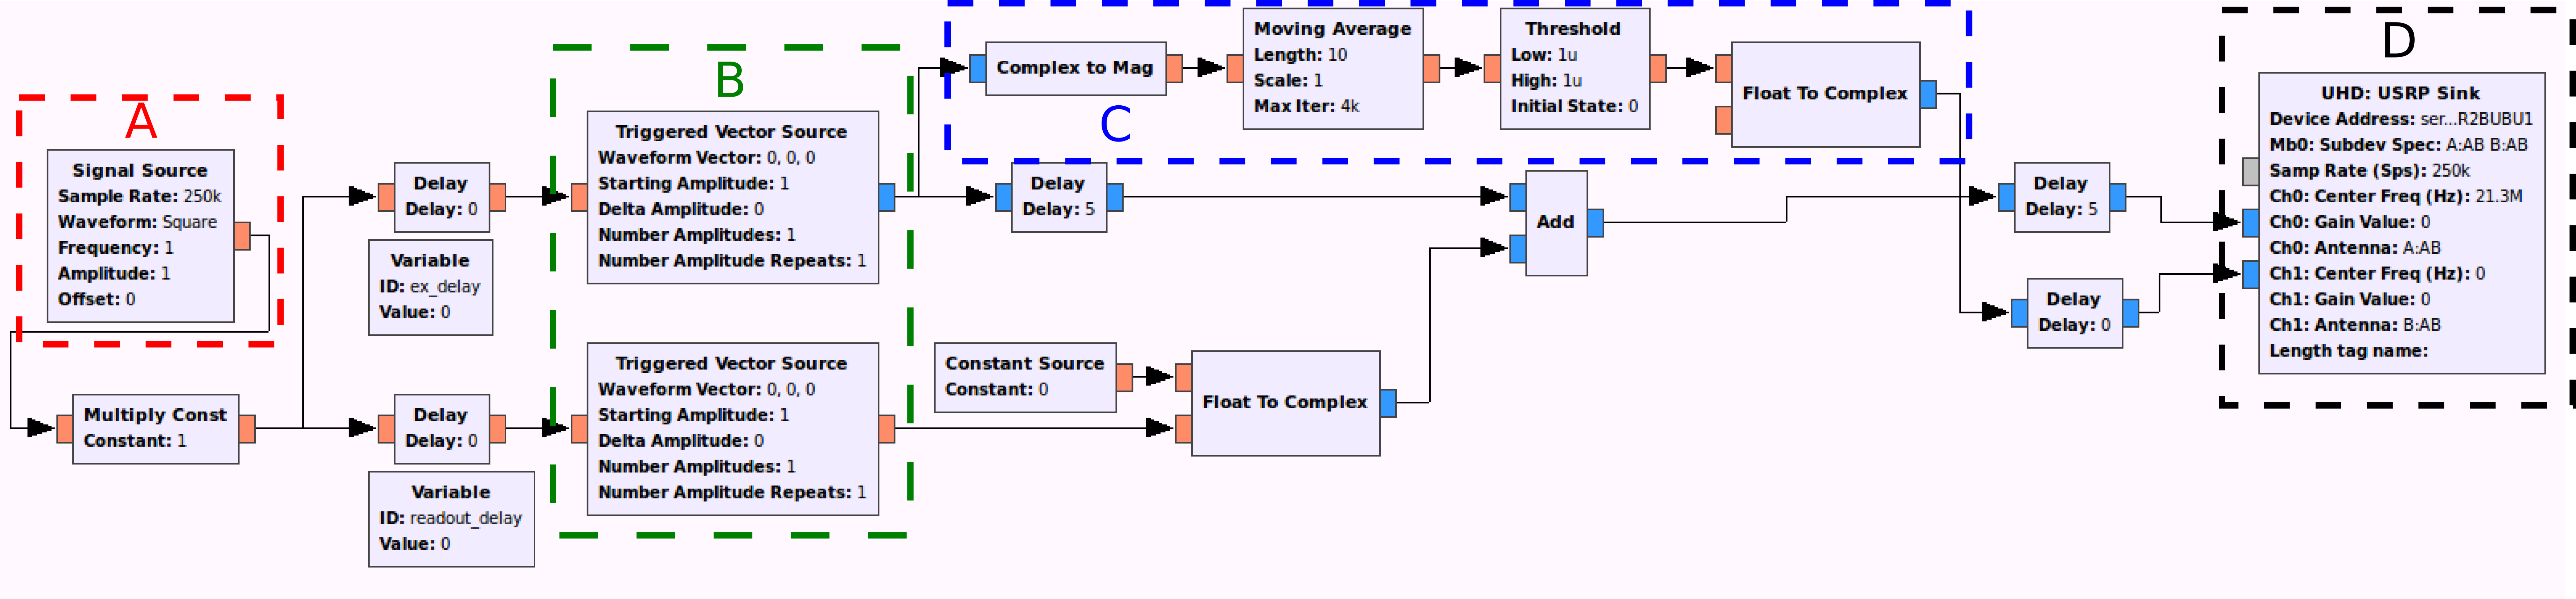
\includegraphics[width = \textwidth,trim=0 0 0 0,clip=false]{fid_tx.png}
\caption{Sequence timing and RF excitation flowgraph of the single-pulse sequence \texttt{FID.py}.
The outlined boxes are: A) The TR square wave signal generator, which triggers all sequence events. 
B) Triggered Vector Sources that generate an RF excitation pulse (top) and a signal recording gate (bottom). 
C) A transmit-enable pulse is generated from the RF excitation pulse to unblank the RF amplifier.
D) The USRP Sink block routes the baseband signals to three channels on the SDR, operating at RF (for the excitation pulse and the signal recording gate) or DC (for the transmit-enable pulse).}
\label{fig:txflow}
\end{center}
\end{figure}

\begin{figure}[ht]
\begin{center}
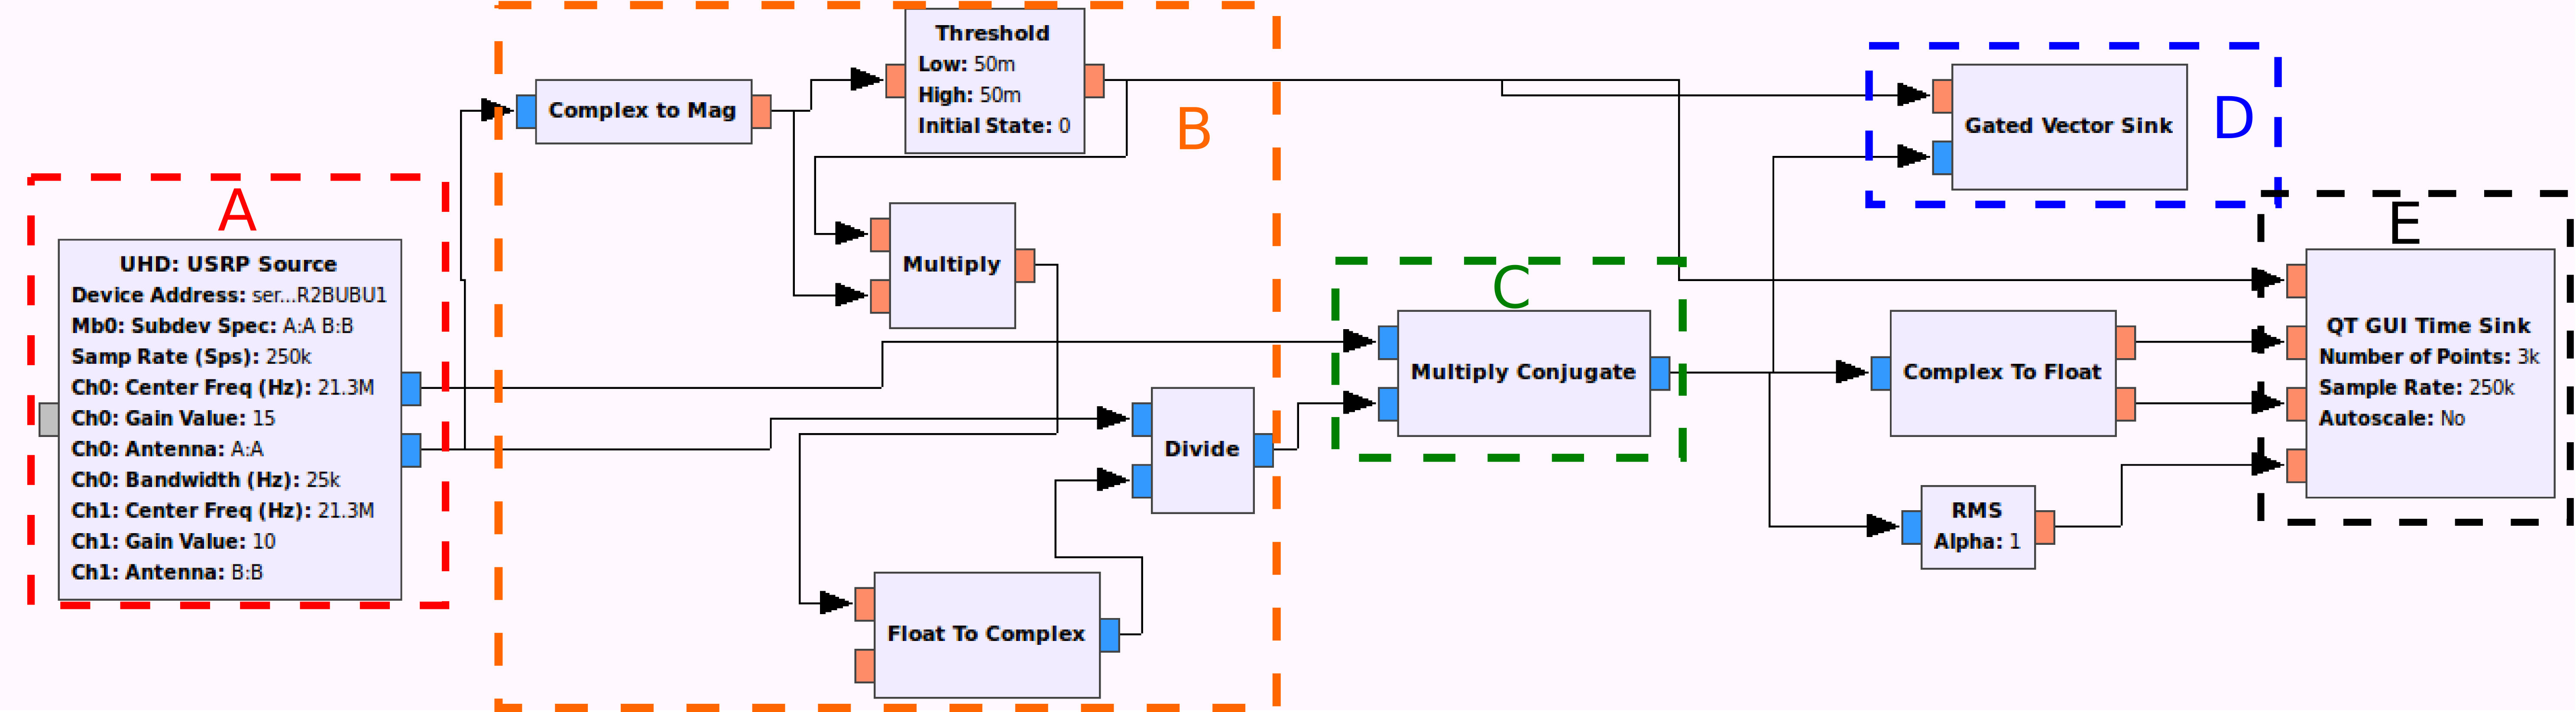
\includegraphics[width = \textwidth,trim=0 0 0 0,clip=false]{fid_rx.png}
\caption{RF Receive flowgraph of the single-pulse sequence \texttt{FID.py}.  The outlined boxes are: A) the USRP
Source, which converts received data into a complex data stream; 
B) a group of blocks used to
normalize the signal recording gate pulse's amplitude while preserving its phase; 
C) a multiply conjugate block that removes the signal recording gate pulse's phase from the FID signal phase to correct phase drifts; 
D) the gated vector sink which stores the raw data to a vector; and E) a QT GUI sink used to display the received signal in real time.}
\label{fig:rxflow}
\end{center}
\end{figure}

\par Figure~\ref{fig:rxflow} shows the receive section of the flowgraph for the single-pulse sequence.  
The far left block in outlined box A is the USRP Source which outputs baseband signals
coming from the SDR's receive channels.  
The bottom data stream from this block is the complex RF data received from the scanner's preamplifier, 
and the top stream is the looped-back signal recording gate pulse, which serves two purposes in the flowgraph.
First, it controls the Gated Vector Sink box D so that the FID signal is only recorded over the desired interval.  
Second, it is used to correct spectrometer phase drifts. 
This is done by the blocks in box B, which normalize the amplitude of signal recording gate pulse, but preserve its phase, and
the received FID signal is multiplied with the normalized signal recording gate pulse's complex conjugate in box C.
This works because the both the excitation and the signal recording gate pulses originated from the same daughterboard with the same phase.
The far right block in box E is a \textit{QT GUI Sink} that is used to display the received signal in real time.  
A representative QT GUI Sink window is shown in Figure~\ref{fig:gui} for the spin echo imaging sequence (described below).

\par The same strategies used to develop the FID single-pulse sequence 
were applied to enable gradient waveform generation for 2D and 3D imaging.
The gr-MRI package includes three common imaging sequences, 
and a template sequence to enable development of new sequences.
These sequences are described next.
The software was built using GNU Radio version 3.7.5.1, 
and uses the scientific Python libraries 
NumPy (http://www.numpy.org) and Matplotlib (http://matplotlib.org).
All communication with SDR's occurs via USRP Sink and Source blocks, 
which in spite of their vendor-specific name are compatible with all SDR's 
that are supported by GNURadio. 
The full package and a detailed user guide can be downloaded at https://bitbucket.org/wgrissom/gnuradio-mri. 
%\textcolor{red}{Also talk about live disc?}

\begin{figure}[!ht]
\begin{center}
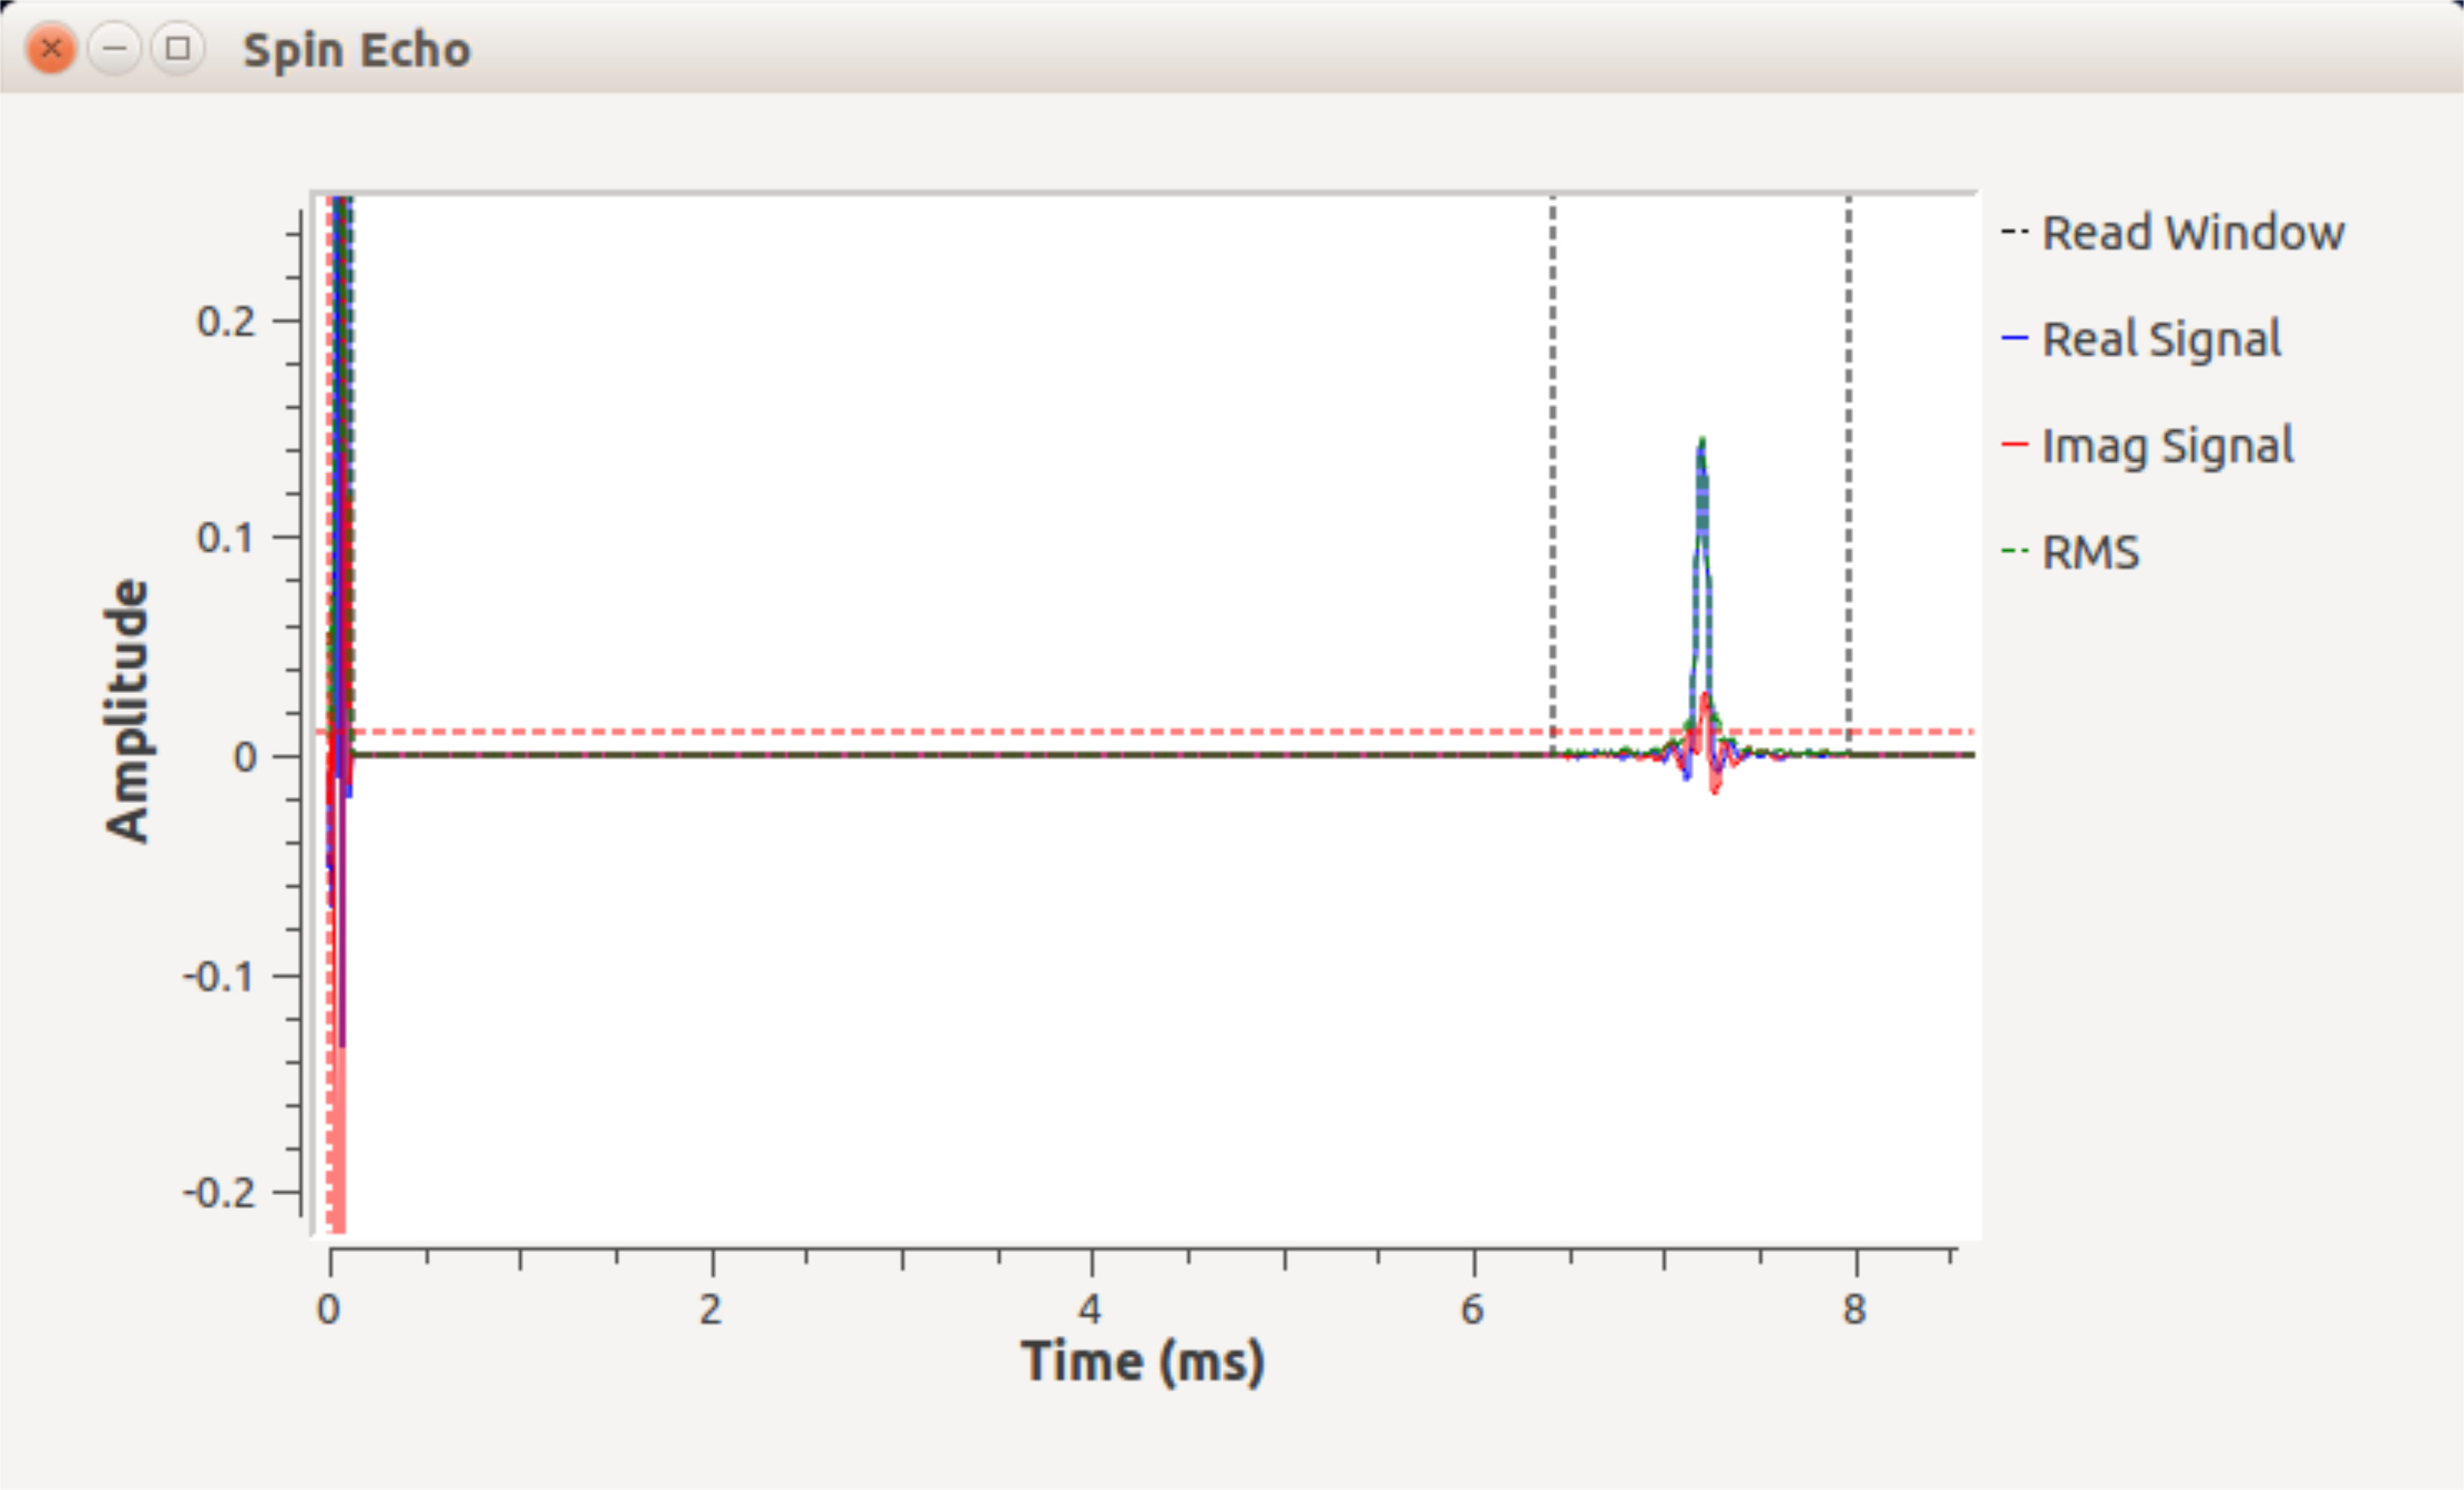
\includegraphics[width = 1\textwidth,trim=0 0 0 0,clip=false]{scan_screenshot.png}
\caption{Screen shot of the receive data shown in the QT GUI window while running the spin echo sequence \texttt{spinecho.py}.}
\label{fig:gui}
\end{center}
\end{figure}

\paragraph{Gradient-recalled echo: \texttt{gradecho.py}}
Figure~\ref{fig:gre_image}a plots the gradient-recalled echo (GRE) pulse sequence 
generated by the script \texttt{gradecho.py}, 
and defines some relevant scan parameters.  
By default the sequence plays a Hamming-windowed sinc excitation pulse
concurrently with a slice-select gradient trapezoid in the $z$ direction to localize the excitation to a slice in the sample.
Phase encoding, slice rewinding and readout prephasor trapezoids occur immediately after the pulse,
followed by the readout gradient and acquisition window which are centered at the echo time (TE). 
Compared to the single-pulse sequence described above, 
the GRE sequence's flow graph includes three more Triggered Vector Sources to generate 
gradient pulse waveforms in three spatial dimensions.

\par Table~\ref{table:sequenceparams} lists the sequence parameters that can be set in the configuration file
\texttt{gre\_config.txt} or during the prescan period before running the scan, 
and Table~\ref{table:sequencefunctions} shows the user-accessible functions defined by \texttt{gradecho.py}
and the other imaging sequences described below.  
Many of the parameters in Table~\ref{table:sequenceparams} also apply to the other sequences,
as indicated. 
All scan parameters set in the config file can be changed dynamically while running the scan by calling \texttt{params.set\_\{param\_name\}(\{value\})}, where \texttt{param\_name} is the name of the parameter to be changed, 
and \texttt{value} is the new value to be assigned.
Each time a parameter is changed, the parameter update functions also update all dependent pulse sequence parameters.
Parameters can be saved to Python pickle (\texttt{.pkl}) files and can also be loaded from pickle files when operating in interactive prescan mode.

\paragraph{Spin echo: \texttt{spinecho.py}}
Figure~\ref{fig:se_image}a plots the spin echo (SE) pulse sequence produced by \texttt{spinecho.py}. 
Compared to the GRE sequence, the SE sequence adds a block refocusing pulse midway between
the excitation pulse and the readout window. 
%Sequence parameters are defined in \textit{spin\_config.txt} and sequence parameters and functions 
%are listed in 
%Tables~\ref{table:sequenceparams} and \ref{table:sequencefunctions}, respectively.

\paragraph{Inversion recovery: \texttt{invrecov.py}}
Figure~\ref{fig:ir_image}a plots the inversion recovery (IR) sequence produced by \texttt{invrecov.py}.
Compared to the SE sequence, 
the IR sequence adds a block inversion pulse played TI (inversion time) seconds before
each excitation and signal readout. 
%Sequence variables set in \textit{invr\_config.txt} and sequence parameters and functions are 
%listed in Tables~\ref{table:sequenceparams} and \ref{table:sequencefunctions}, respectively.

\begin{table}
%\begin{center}
\begin{tabularx}{\textwidth}{|c|X|c|c|}
	\hline
	\textbf{Param Name} & \textbf{Param Description} & \textbf{Units} & \textbf{Sequence}  \\ \hline
	\texttt{TR} & Repetition time & s &GRE,SE,IR,FID\\ \hline
	\texttt{CF} & Center frequency & Hz &GRE,SE,IR,FID\\ \hline
	\texttt{offset} & Center frequency Offset & Hz & GRE,SE,IR,FID\\ \hline
	\texttt{p90} & Excitation pulse length & s & GRE,SE,IR,FID\\ \hline
	\texttt{p180} & Refocusing pulse length & s & SE,IR\\ \hline
	\texttt{TE} & Echo time & s & GRE,SE,IR\\ \hline
	\texttt{TI} & Inversion time & s & IR\\ \hline
	\texttt{BW} & Readout bandwidth & Hz & GRE,SE,IR\\ \hline
	\texttt{readout\_length} & FID Readout length & s & FID \\ \hline
	\texttt{NRO} & Matrix dimension in readout direction & integer & GRE,SE,IR\\ \hline
	\texttt{NPE} & Number of phase encodes & integer & GRE,SE,IR\\ \hline
	\texttt{FOVread} & Field of view in readout dimension & mm & GRE,SE,IR\\ \hline
	\texttt{FOVphase} & Field of view in phase encode dimension & mm & GRE,SE,IR\\ \hline
	\texttt{readdir} & Readout dimension (x=1,y=2,z=3) & integer & GRE,SE,IR\\ \hline
	\texttt{phasedir} & Phase encode dimension & integer & GRE,SE,IR\\ \hline
	\texttt{slicedir} & Slice dimension & integer & GRE,SE,IR\\ \hline
	\texttt{pre\_dur} & Readout prephasor duration & s & GRE,SE,IR\\ \hline
	\texttt{phase\_dur} & Phase encode gradient duration & s & GRE,SE,IR\\ \hline
	\texttt{rewinder\_length} & Slice gradient rewinder length & s & GRE,SE,IR\\ \hline
	\texttt{slice\_thick} & Slice thickness & mm & GRE,SE,IR\\ \hline
	\texttt{nav} & Number of averages & integer & GRE,SE,IR,FID\\ \hline
	\texttt{TBW} & Excitation pulse time-bandwidth product & unitless & GRE,SE,IR\\ \hline
	\texttt{slice\_shift} & Slice offset & Hz & GRE,SE,IR\\ \hline
	\texttt{ex\_type} & Excitation pulse shape (Square=0, Sinc=1) & integer & GRE,SE,IR\\ \hline
	\texttt{ischopped} & RF Chopping (Off=0, On=1) & integer & GRE,SE,IR\\ \hline
	\texttt{interactive\_mode} & Pre-scan/Interactive mode (Off=0, On = 1) & integer & GRE,SE,IR\\ \hline
	\texttt{param\_file} & .pkl file name for automatically loaded scan parameters & string & GRE,SE,IR,FID\\ \hline
	\texttt{leader\_ID} & ``Leader'' radio serial ID (not interactive) & string & GRE,SE,IR,FID\\ \hline
	\texttt{follower\_ID} & ``Follower'' radio serial ID (not interactive) & string & GRE,SE,IR,FID\\ \hline
	
\end{tabularx}
\caption{Parameters that can be adjusted dynamically or in configuration files for each of the pulse sequences.}
\label{table:sequenceparams}
%\end{center}
\end{table}

\begin{table}
\begin{tabularx}{\textwidth}{|c|X|X|}
	\hline
	\textbf{Function} & \textbf{Description} & \textbf{Argument}\\ \hline
	\texttt{params.set\_\{param\}(value)} & Change value of parameter \texttt{\{param\}} and dependents & \texttt{value}: new value of parameter \\ \hline
	\texttt{params.param\_table()} & Display current sequence parameters & None \\ \hline
	\texttt{sync()} & Synchronize two radios & None \\ \hline
	\texttt{read\_on()} & Enable readout gradient & None \\ \hline
	\texttt{slice\_on()} & Enable slice select gradient & None \\ \hline
	\texttt{grads\_off()} & Disable all gradients & None \\ \hline
	\texttt{profile()} & Display 1D object profile with \texttt{params.nav} number of averages & None\\ \hline
	\texttt{show\_pulses()} & Plot pulse sequence & None \\ \hline
	\texttt{params.save\_params(file)} & Save scan parameters to pickle file & \texttt{file}: file name to save parameters to\\ \hline
	\texttt{params.import\_params(file)} & Import scan parameters from pickle file & \texttt{file}: file name to load parameters from\\ \hline
	\texttt{calib\_slice()} & Calibrate slice gradient rewinder & None \\ \hline
	\texttt{calib\_readout()} & Calibrate readout gradient prephasor to center signal & None \\ \hline
	\texttt{run()} & Run imaging sequence and record data & None \\ \hline
	\texttt{data.recon()} & Reconstruct image & None \\ \hline
	\texttt{end()} & Stop sequence and program & None\\ \hline	
\end{tabularx}
\caption{User interface functions defined by the three imaging pulse sequences.}
\label{table:sequencefunctions}
\end{table}

\paragraph{Template sequence: \texttt{template.py}} 
gr-MRI also provides a template sequence to enable rapid development of custom pulse sequences.  
The template is based on \texttt{gradecho.py}, 
and is heavily commented to give instructions for how to edit the sequence.  
In the simplest case, the user need only define the RF pulse shape to generate a pulse sequence, 
however the user can define custom gradient waveforms, and new data acquisition windows if desired; 
multiple windows could also be defined for multi-echo sequences.  
The template includes function definitions that provide the same functionality as the full imaging pulse sequences, 
and the config file is preloaded with general parameter names that were used in the those pulse sequences.

\subsection*{System calibrations}

\paragraph{Transmit/Receive Delay} 
Since a single SDR typically does not provide sufficient channels for an MRI scan, 
gr-MRI imaging sequences presume the use of two radios, 
one for generating RF waveforms and one for generating gradient waveforms. 
Due to transmit delays resulting from USB latency which can be on the order of 20 ms, 
radio synchronization is essential while running these two-radio pulse sequences.  
To address this, one radio is designated the `leader' and the other the `follower'.
It is assumed that the leader radio will produce the RF pulses and transmit enable 
pulse and the follower radio will generate the gradient waveforms.
The gr-MRI sequences use a port on each radio to loop back a ten sample block synchronization pulse into dedicated receive channels on the follower SDR three times per TR.
Figure~\ref{fig:syncflow} shows how these signals are processed in the sequence flowgraphs.
The received synchronization pulses are each thresholded 
and combined as the real and imaginary parts of a single complex signal that is stored in a Vector Sink.  
While running a scan, 
a function in the imaging sequence script continuously checks the synchronization data from the 
Vector Sink three times per TR to compare the pulse timings.
If a desynchronization is detected, 
the function pauses the main pulse sequence and 
sets global leader and follower delays to realign the transmitted pulses.
When operating in interactive mode, 
the user can resynchronize the radios at any time by calling the  \texttt{sync()} function.
Desynchronization during data acquisition may corrupt the received data; 
the frequency with which desynchronization events 
occur with our setup was characterized as described below.

\begin{figure}[ht]
\begin{center}
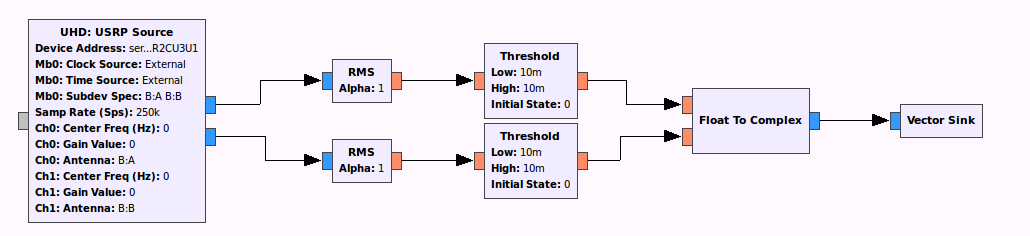
\includegraphics[width = \textwidth,trim=0 0 0 0,clip=false]{sync_flow.png}
\caption{Synchronization section of the imaging sequence flowgraphs.}
\label{fig:syncflow}
\end{center}
\end{figure}

\paragraph{Center Frequency and Transmit Voltage} Automatic center frequency and power
calibration functions are implemented as part of the \texttt{FID.py} pulse sequence, 
and are listed in Table \ref{table:calib_functions}.
The center frequency offset calibration function is illustrated in Figure~\ref{fig:calib}a.  
The user specifies the desired number of signal averages to use for FID measurement, 
and the system displays the resultant FFT of the averaged signal, along with a fit Lorentzian curve.
The new center frequency offset is defined to be the frequency corresponding to the peak of the Lorentzian curve, 
and is set automatically when the script has completed.  
This calibration can be run multiple times for best accuracy, 
since SNR increases as the radio's frequency approaches the Larmor frequency.
The power calibration, illustrated in Figure~\ref{fig:calib}b, 
finds the necessary RF pulse amplitude to achieve a 90 degree flip angle for a fixed-duration block pulse.  
The user specifies the desired number of signal averages, 
and the script acquires signals across a range of pulse amplitudes until a maximum received signal amplitude has been reached.
Both functions save the optimized parameters to a Python pickle file named \texttt{cal.pkl} 
which is loaded and used by the imaging pulse sequences.  

\begin{table}
\begin{tabularx}{\textwidth}{| c | X | c |}
	\hline
	\textbf{Function} & \textbf{Description} & \textbf{Argument}  \\ \hline
	\texttt{calibrate\_offset(nav)} & Find offset from true center frequency to default center frequency & \texttt{nav}: number of averages\\ \hline
	\texttt{calibrate\_power(nav)} & Find the optimal excitation pulse amplitude needed to excite a 90 degree flip angle & \texttt{nav}: number of averages\\ \hline
	\texttt{save\_calib()} & End calibration flow graph and saves calibration data to \texttt{cal.pkl} & None\\ \hline	
\end{tabularx}
\caption{Center frequency and power calibration functions implemented in \texttt{FID.py}.}
\label{table:calib_functions}
\end{table}


\begin{figure}[!ht]
\begin{center}
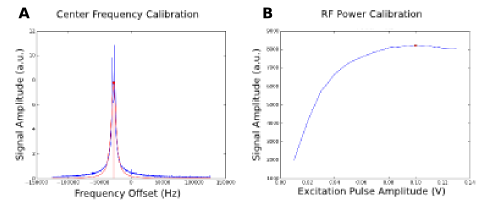
\includegraphics[width = .75\textwidth,trim=0 0 0 0,clip=false]{calibration.png}
\caption{User-visible plots that appear when running (A) the center frequency calibration function, and (B) the 90 degree pulse power calibration function. Both are defined in \texttt{FID.py}.}
\label{fig:calib}
\end{center}
\end{figure}

\paragraph{Gradient strength} 
The gr-MRI package also provides a gradient strength calibration script called \texttt{grad\_calibration.py}, 
which uses a spin echo sequence to measure one-dimensional profiles of an object of known size.  
The user defines the gradient dimension to calibrate, and the object size in that dimension.
The sequence then calibrates the gradient strength as a function of radio output voltage based on pre-loaded gradient amplitudes 
and the resultant frequency bandwidth of object's profile.  
Gradient strengths are saved in units of Gauss/mm/Volt to the file \texttt{gcal.pkl} and are 
used by the imaging sequences to convert desired image FOV 
and matrix size parameters gradient pulse amplitudes and step sizes.
Table~\ref{table:gradcalib_functions} shows all of the functions available to the user when running the \texttt{gradcalib.py} script.
This calibration should only need to be done once for a given scanner. 

\begin{table}
\begin{tabularx}{\textwidth}{| c | X | c |}
	\hline
	\textbf{Function} & \textbf{Description} & \textbf{Inputs}  \\ \hline
	\texttt{sync()} & Synchronize the outputs of two radios. & None\\ \hline
	\texttt{grad\_calib(direction)} & Asks for phantom size in specified dimension and calibrates the gradient strength & \texttt{direction}: \texttt{x}, \texttt{y} or \texttt{z}\\ \hline
	\texttt{save\_calib()} & End the calibration flow graph and save calibration data to \texttt{gcal.pkl} & None\\ \hline	
\end{tabularx}
\caption{Gradient calibration functions defined by the gradcalib.py script.}
\label{table:gradcalib_functions}
\end{table}


\subsection*{Data processing and image reconstruction}
%There are two classes created and accessed by each imaging sequence.
%The first class is called \texttt{params} and contains scan parameters that were specified in the configuration files, 
%additional scan parameters derived from calibration files, and generated pulses for each imaging sequence.
All data from a sequence is automatically transferred to an object of class \texttt{data} after a sequence is run.
The object contains the raw data from the sequence's Gated Vector Sink, 
and a time stamp indicating when the sequence was initiated.
When the \texttt{data.recon()} function is called, the data is reformatted (and averaged, if 
averaging was performed) to create an \texttt{NPE}$\times$\texttt{NRO} matrix. If the 
readout dimension was oversampled with respect to the desired readout bandwidth, the 
matrix is decimated to the specified matrix size using a 60 tap anti-aliasing FIR
filter. Finally, a 2D inverse FFT reconstruction is performed, which corrects for RF 
chopping if it is present. The formatted k-space data matrix is returned in 
\texttt{data.kdata} and the image is returned in \texttt{data.imdata}.


%\begin{figure}[ht]
%\begin{center}
%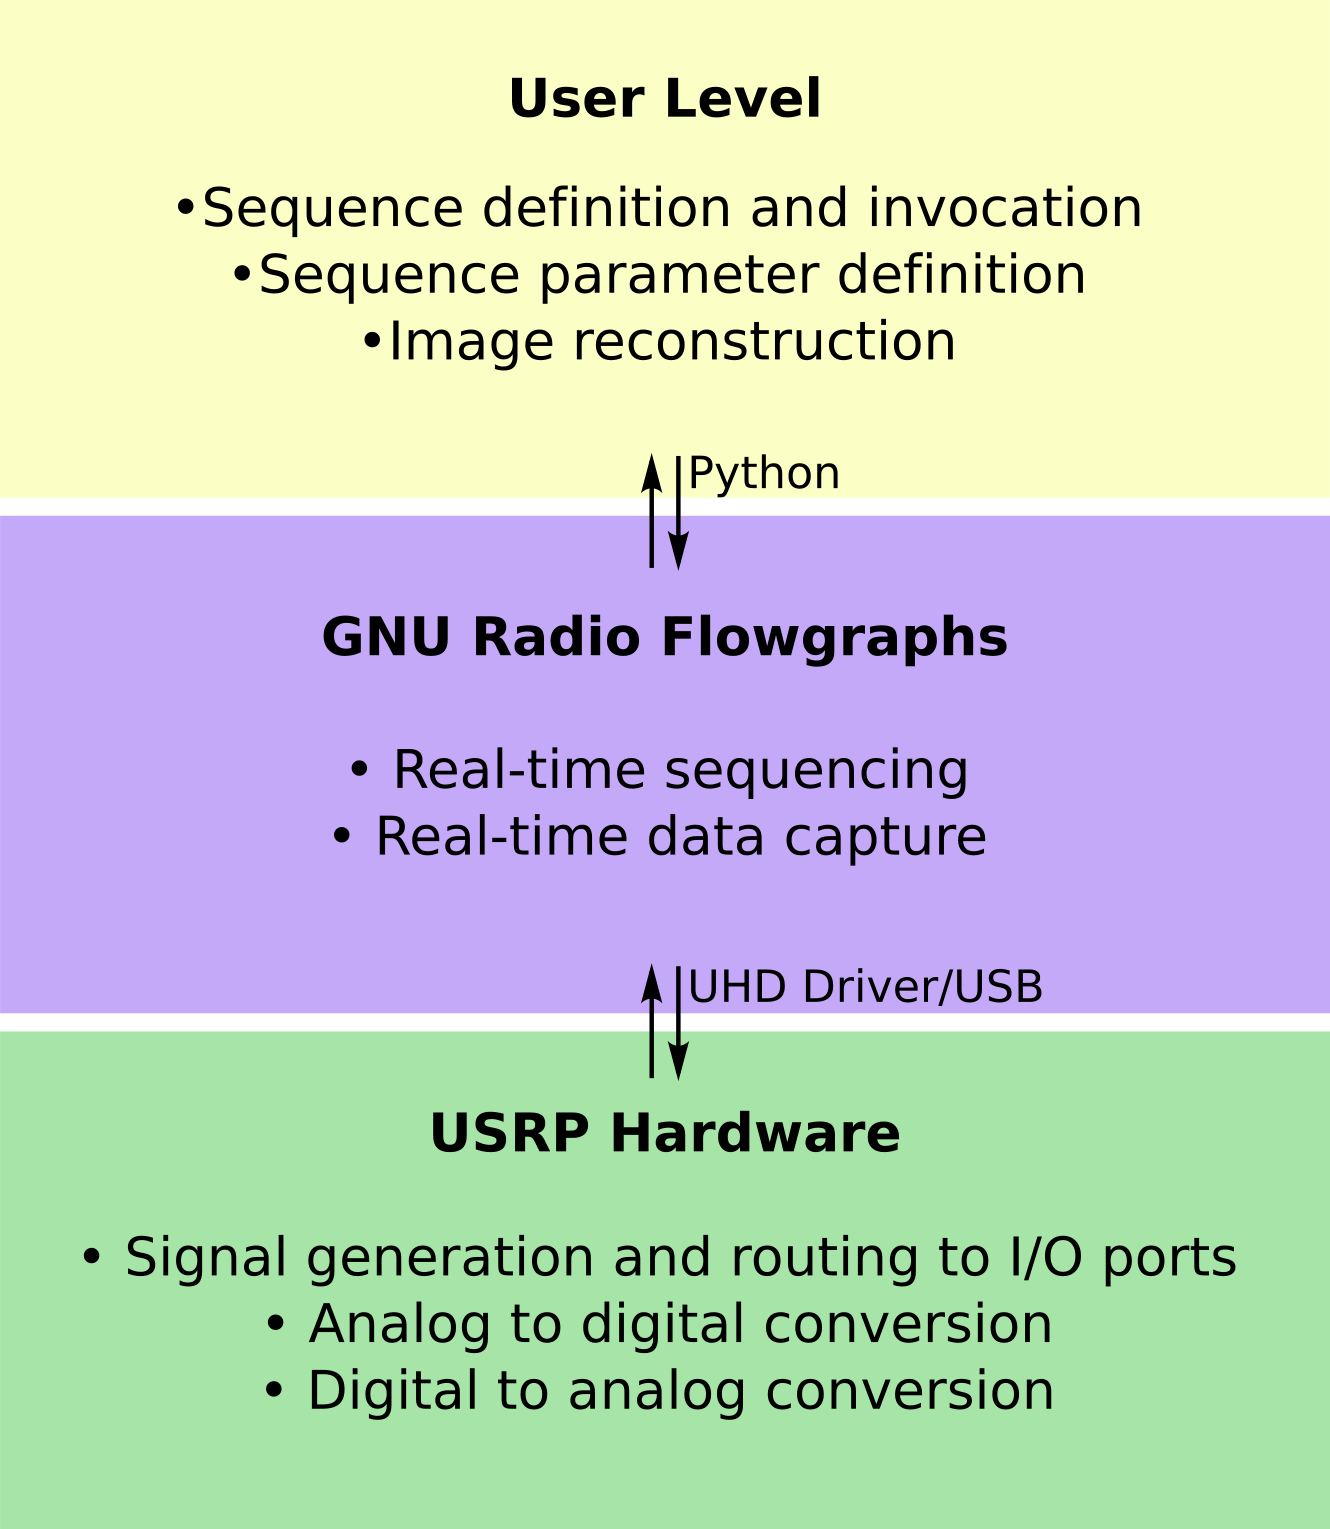
\includegraphics[width = .5\textwidth,trim=0 0 0 0,clip=false]{overview.png}
%\caption{{High level organization of the gr-MRI software package.}}
%\label{fig:overview}
%\end{center}
%\end{figure}

\begin{figure}[!ht]
\begin{center}
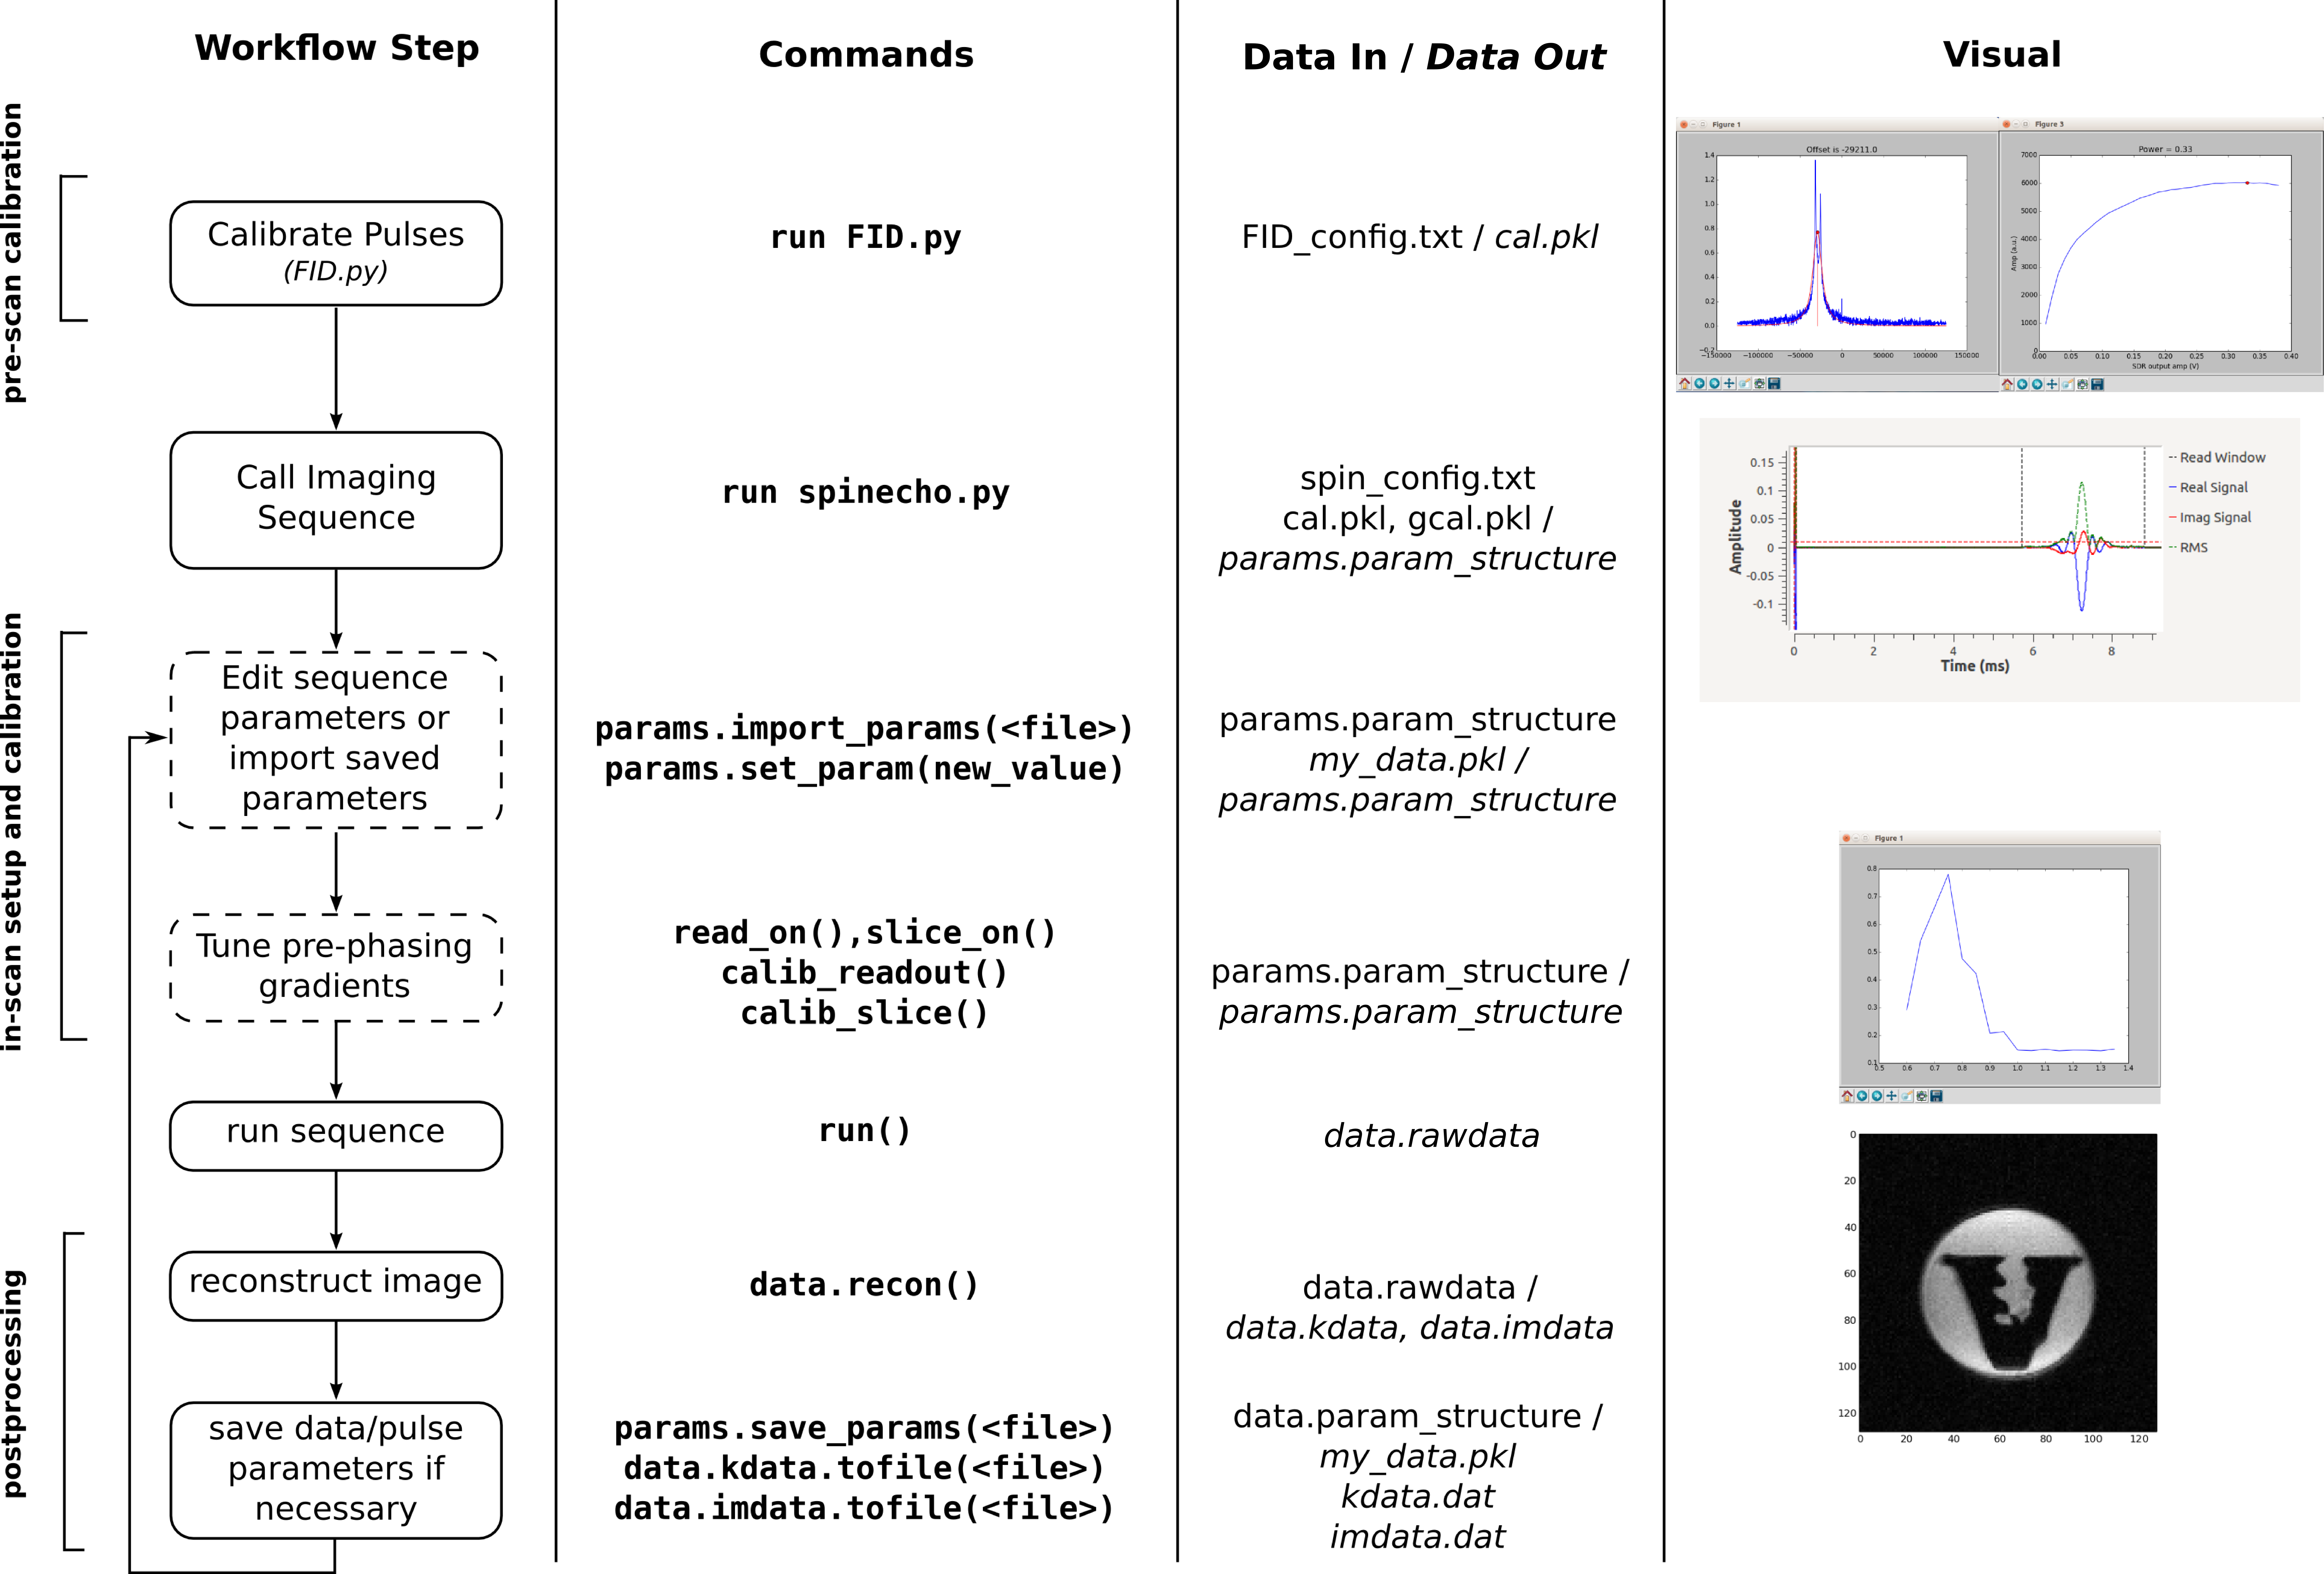
\includegraphics[width = \textwidth,trim=0 0 0 0,clip=false]{workflow.png}
\caption{Workflow illustration for the \texttt{spinecho.py} imaging sequence.  
Dotted lines in the workflow steps indicate optional steps that can be turned on or off using the \texttt{interactive\_mode} parameter in the configuration file.  
The second column shows commands 
as the user would enter them into the IPython shell.  
The third column describes the data that is used or produced by each command, 
and the fourth column shows any images or plots that are created.}
\label{fig:workflow}
\end{center}
\end{figure}

\subsection*{Workflow summary}
Figure \ref{fig:workflow} summarizes the workflow implemented by gr-MRI, 
for the \texttt{spinecho.py} imaging sequence.  
The diagram shows a workflow step, 
and the output that the step affects and (where applicable) the input the step receives.  
A gr-MRI imaging experiment comprises the following steps: 
\begin{enumerate}
\item RF power and center frequency parameters are determined and saved using \texttt{FID.py} as described in the calibration section above.  
\item The user updates the imaging sequence's config file with the desired pulse sequence parameters for their scan.  
In this case, the config file is named \texttt{spin\_config.txt}.  
The user saves the file to commit parameter changes,
and invokes the imaging sequence script (\texttt{spinecho.py}).  
The calibrated parameters from Step 1 are automatically loaded, as well as the parameters 
from the sequence's config file. 
\item Interactive Mode starts and the raw signal is displayed in real-time, 
while the user dynamically adjusts sequence parameters or loads saved parameters to see how the parameter changes affect the signal. 
This step is optional.
\item The user can fine-tune the gradient pulse moments 
to center the signal in the acquisition window.
The figure for the ``Tune pre-phasing gradients'' step of Figure \ref{fig:workflow} shows an example of a plot that is shown when tuning the slice gradient.
The plot is integrated signal amplitude versus 
a parameter \texttt{rephase\_fudge}, 
which is calibrated by the script and is 
multiplied by the slice rephasing gradient.
The maximum point on this plot corresponds to the scaling of the rephasing gradient amplitude needed to fully cancel the through-slice phase.
This step is optional but was required periodically on our scanner due to gradient amplifier nonlinearity, 
and may not be necessary on other scanners.
\item The user runs the sequence.
The raw signal from each acquired line of k-space is displayed in the GNU Radio window so the user can monitor the scan.  
The script also outputs the current phase encode line of acquisition, so the user can monitor scan progress.  
\item After the scan has completed, the user can save the raw k-space data for external reconstruction, 
or call \texttt{data.recon()}, to reconstruct an image.  
\item The user can save data or parameters, 
change parameters, or begin a new scan.
\end{enumerate}

\subsection*{Experiments}\label{Experiments}
Experiments were performed on a Maran 0.5 Tesla Oxford Maran tabletop scanner (Resonance Instruments, Witney, U.K.)
to verify the imaging sequences and other functions of the gr-MRI software. 
The software ran on a PC running Ubuntu 14.04 (Canonical, London, U.K.), 
with 16 GB RAM and a 4 GHz Intel Core i7-4790 CPU (Intel Corp, Santa Clara, CA, U.S.A.).
Prior to imaging scans, gradient calibration was performed using a
1$\times$1$\times$1 cm$^3$ cube phantom filled with CuSO\textsubscript{4}-doped water.

\paragraph{SDR Hardware}
All imaging scans used two Ettus Research USRP1 SDRs with connected clocks.
Although the radios perform separate functions, there is a significant difference between the clock speed of individual radios.
This results in a significant time drift between the two radios, 
which would be impractical to correct by the \texttt{sync()} function alone.
We therefore connected the clocks following instructions provided on the GNU Radio website.
The USRP1 comprises an Altera Cyclone FPGA,
a 14 bit (-1 V to 1 V), 128 Ms/sec digital to analog converter,
and a 12 bit (-1 V to 1 V), 64 Ms/sec analog to digital converter.
The USRP1 can accommodate up to two transmit daughterboards and two receive daughterboards, 
each of which provides two channels.  
Each daughterboard can be driven at a unique frequency.
The device connects to the PC running GNU Radio over USB.
In our experiments the leader radio produced the RF excitation pulse and the signal recording gate pulse on one transmit daughterboard, 
and DC transmit-enable and synchronizing pulses on a second transmit daughterboard.
The follower radio produced the gradient pulses and another synchronizing pulse.
Table~\ref{table:hardware} shows the mapping between imaging sequence pulses and ports. 
The naming convention for the channel used is \textit{TX/RX Daughterboard\_Slot A/B\_Channel A/B}. 
%Each pulse and its scheduling was defined in the gr-MRI software package and sent to GNU Radio, 
%where the pulse was mapped to a physical port.
Because the USRP1 produces a maximum pulse amplitude of 1 V 
but our RF amplifier required at least 3.3 V to unblank,
the transmit-enable pulse was used to drive a transistor switch that connected the SDR's 6 V power supply to the RF amplifier's unblanking input.

\begin{table}
\begin{tabular}[c]{| c | c | c | c |}
	\hline
	\textbf{Pulse} & \textbf{Radio/Channel} & \textbf{Input/Output} & \textbf{Destination} \\ \hline
	RF Excitation & Leader TX\_A\_A & Output & RF Amplifier\\ \hline
	Signal recording & Leader TX\_A\_B & Output & Leader RX\_B\_B\\ \hline
	Transmit-enable & Leader TX\_B\_A & Output & RF Amplifier\\ \hline
	Leader sync & Leader TX\_B\_B & Output & Follower RX\_B\_B\\ \hline
	RF Receive & Leader RX\_A\_A & Input & PC \\ \hline
	Gx Gradient & Follower TX\_B\_B & Output & Gradient Amplifier\\ \hline
	Gy Gradient & Follower TX\_A\_B & Output & Gradient Amplifier\\ \hline
	Gz Gradient & Follower TX\_A\_A & Output & Gradient Amplifier\\ \hline
	Follower Sync & Follower TX\_B\_A & Output & Follower RX\_B\_A\\ \hline
\end{tabular}
\caption{Mapping of pulse waveforms to transmit and receive ports on the two SDRs used for the imaging experiments.
The leader SDR generated and received all RF signals,
and the follower SDR generated all gradient pulses.}
\label{table:hardware}
\end{table}

\paragraph{Imaging Scans}
Spin Echo, Gradient Echo, and Inversion Recovery Spin Echo imaging experiments were run with
the sequence parameters shown in Table~\ref{table:parameters}.
All scans used RF chopping to move DC artifacts to the edge of the FOV, 
and images were reconstructed using gr-MRI's 2D inverse FFT reconstruction. 
All sequences were used to image an 11 $\times$ 8 mm$^2$ 3D-printed Vanderbilt University logo shaped phantom
immersed in a 15 mm NMR tube filled with sunflower seed oil.
The spin echo acquisitions were repeated 15 times with and without running interactive mode first,
to record the number of leader-follower desynchronization events.
The inversion recovery scan was repeated eight times with TI's of
10, 25, 50, 100, 150, 200, 300, and 400 ms. 

\paragraph{Frequency-swept pulse generation}
To validate the software and the SDR's ability to generate frequency-swept waveforms, 
an experiment was performed in which a Triggered Vector Source was used to 
produce a frequency-swept waveform originally designed for Bloch-Siegert $B_1^+$ mapping \cite{janki:2013} (Figure \ref{fig:f_sweep}, left).
The small signal RF pulse was looped back into a USRP1 receive channel and recorded.
For comparison, the same waveform was generated using the Maran scanner's spectrometer,
and recorded the same way.

\begin{table}
\begin{tabular}[c]{| c | c | c | c | c | c | c | c | c | c |}
	\hline
	\textbf{Imaging Parameter} & \textbf{Spin Echo} & \textbf{Gradient Echo} & \textbf{Inversion Recovery} \\ \hline
	Sequence script & \texttt{spinecho.py} & \texttt{gradecho.py} & \texttt{invrecov.py} \\ \hline
	TE (ms) & 10 & 1.5 & 10\\ \hline
	TR (ms) & 1000 & 1000 & 750\\ \hline
	Flip angle (degrees) & 90 & 90 & 90\\ \hline
	Matrix size & 128$\times$128 & 128$\times$128 & 128$\times$128\\ \hline
	FOV (mm) & 20$\times$20 & 20$\times$20 & 20$\times$20\\ \hline
	Slice Thickness (mm) & 4 & 4 & 5\\ \hline
	BW (kHz) & 41.7 & 41.7 & 41.7\\ \hline
	Averages & 3 & 3 & 3\\ \hline
\end{tabular}
\caption{Parameters for each imaging scan.}
\label{table:parameters}
\end{table}  


\section*{Results}

\begin{figure}[h]
\begin{center}
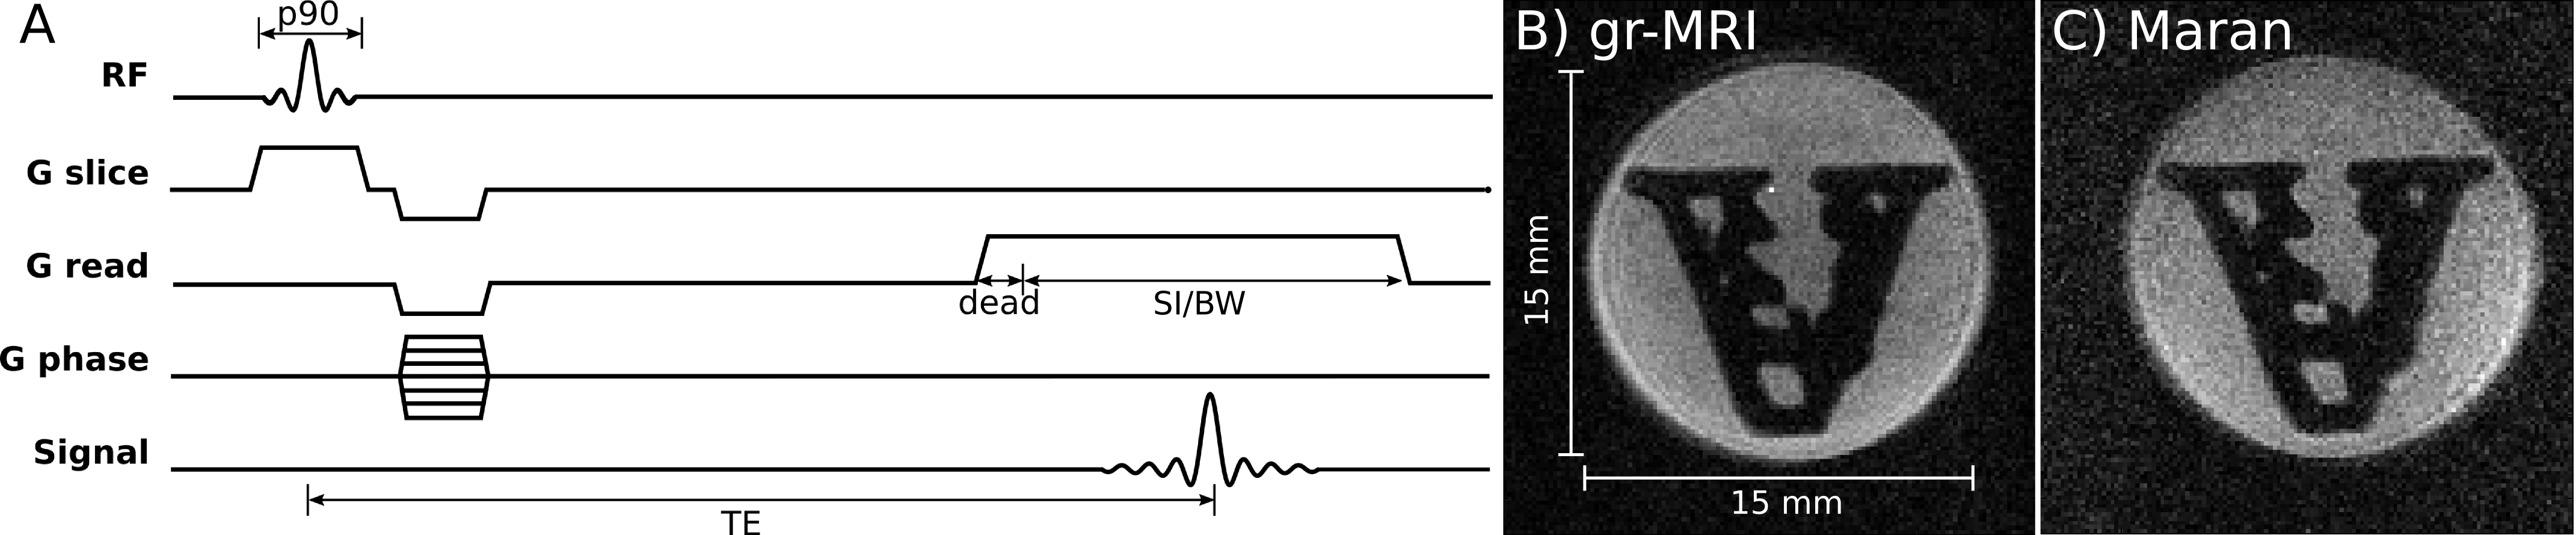
\includegraphics[width = 1\textwidth,trim=0 0 0 0,clip=false]{GRE_results.png}
\caption{{(A) Slice-selective gradient-recalled echo pulse sequence generated by \texttt{gradecho.py}.
(B) A 128 $\times$ 128 image acquired with 4 mm slice thickness.  
Arrows indicate chemical shift artifacts in the frequency-encoded (horizontal) dimension.
(C) Comparable gradient-recalled echo image acquired using the Maran spectrometer.}}
\label{fig:gre_image}
\end{center}
\end{figure}
 
\begin{figure}[h]
\begin{center}
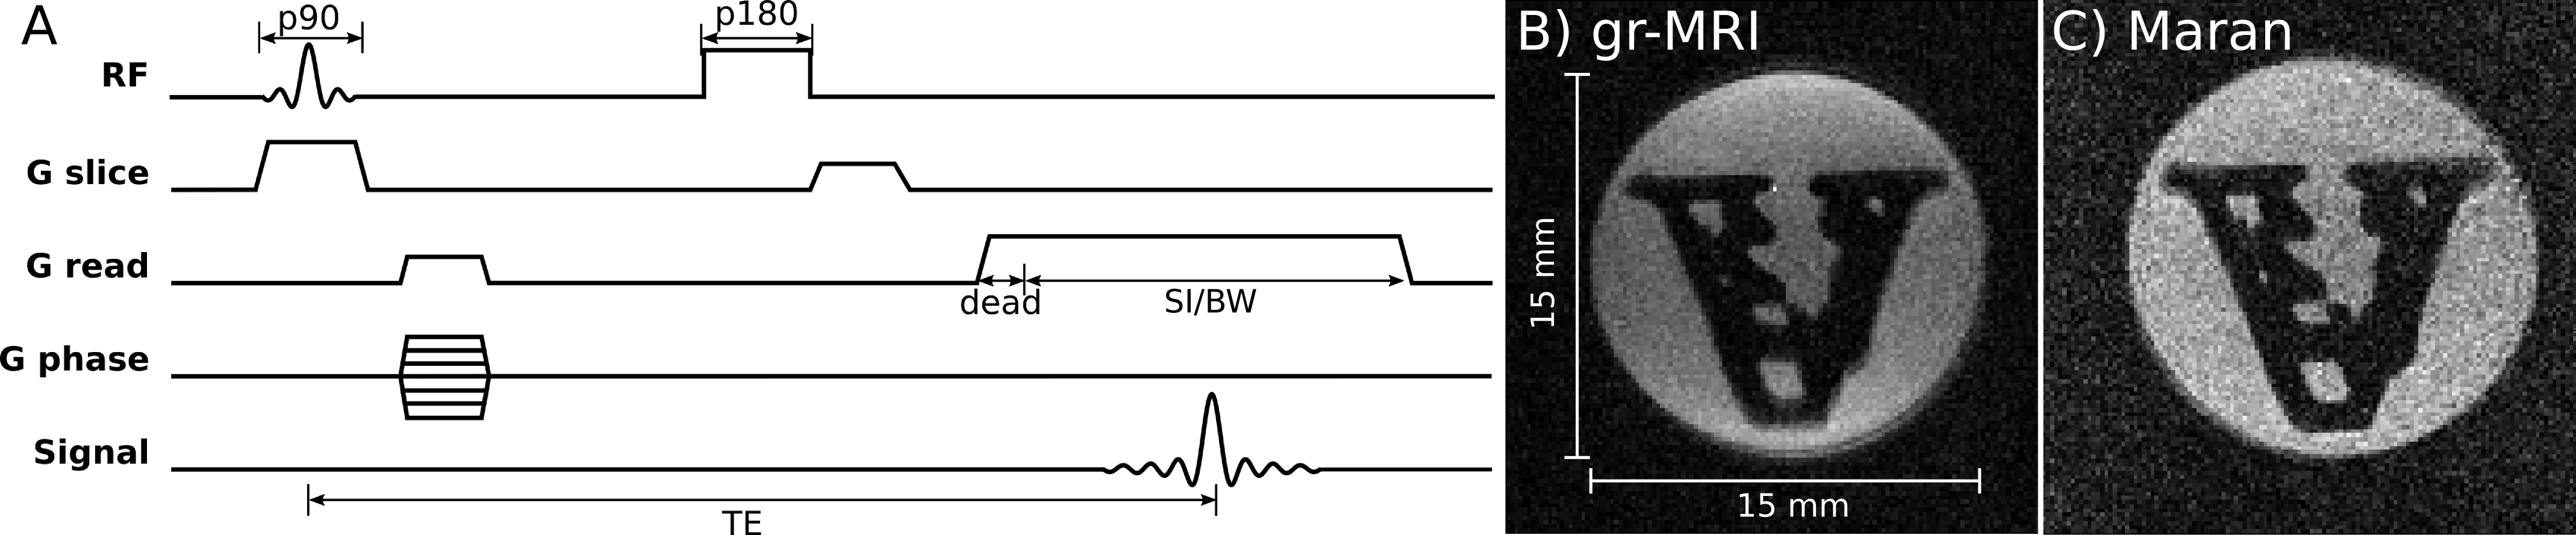
\includegraphics[width = 1\textwidth,trim=0 0 0 0,clip=false]{SE_results.png}
\caption{{(A) Slice-selective spin echo pulse sequence generated by \texttt{slicespin.py}.
(B) A 128$\times$128 image acquired with 4 mm slice thickness. 
The arrow indicates a small chemical shift artifact in the frequency-encoded (horizontal) dimension. 
(C) Comparable spin echo image acquired using the Maran spectrometer.}}
\label{fig:se_image}
\end{center}
\end{figure}
 
\subsection*{Imaging} Figure~\ref{fig:gre_image}B shows the image acquired with \texttt{gradecho.py},
and Figure~\ref{fig:gre_image}C shows a gradient echo image acquired using the Maran spectrometer with closely-matched parameters.
A visual comparison of the images confirms a lack of geometric distortions in the gr-MRI image,
other than some blurring due to chemical shift in the frequency-encoded (horizontal) direction (indicated by the arrows). 
The Maran chemical shift was in the opposite direction because the polarity of the readout gradient was opposite that of the SDR.
The phantom dimensions measured from the gr-MRI image are 15.15 and 15.28 mm, 
which are close to the expected 15 mm dimensions.
Figure~\ref{fig:se_image}B shows the image acquired with \texttt{spinecho.py}, and
Figure~\ref{fig:se_image}C shows a spin echo image acquired using the Maran spectrometer.
A visual comparison of the images confirms a lack of geometric distortions in the gr-MRI image,
other than some blurring due to chemical shift in the frequency-encoded (horizontal) direction (indicated by the arrows).
The phantom dimensions measured from the gr-MRI image are 15.25 and 14.85 mm, 
which again are close to the expected 15 mm dimensions.
Figure~\ref{fig:ir_image}B shows images acquired across a range of TIs in the 15 mm oil phantom.  
The signal is nulled at approximately 100 ms, 
which is consistent with the expected oil $T_1$ of approximately 150 ms.

\begin{figure}[h]
\begin{center}
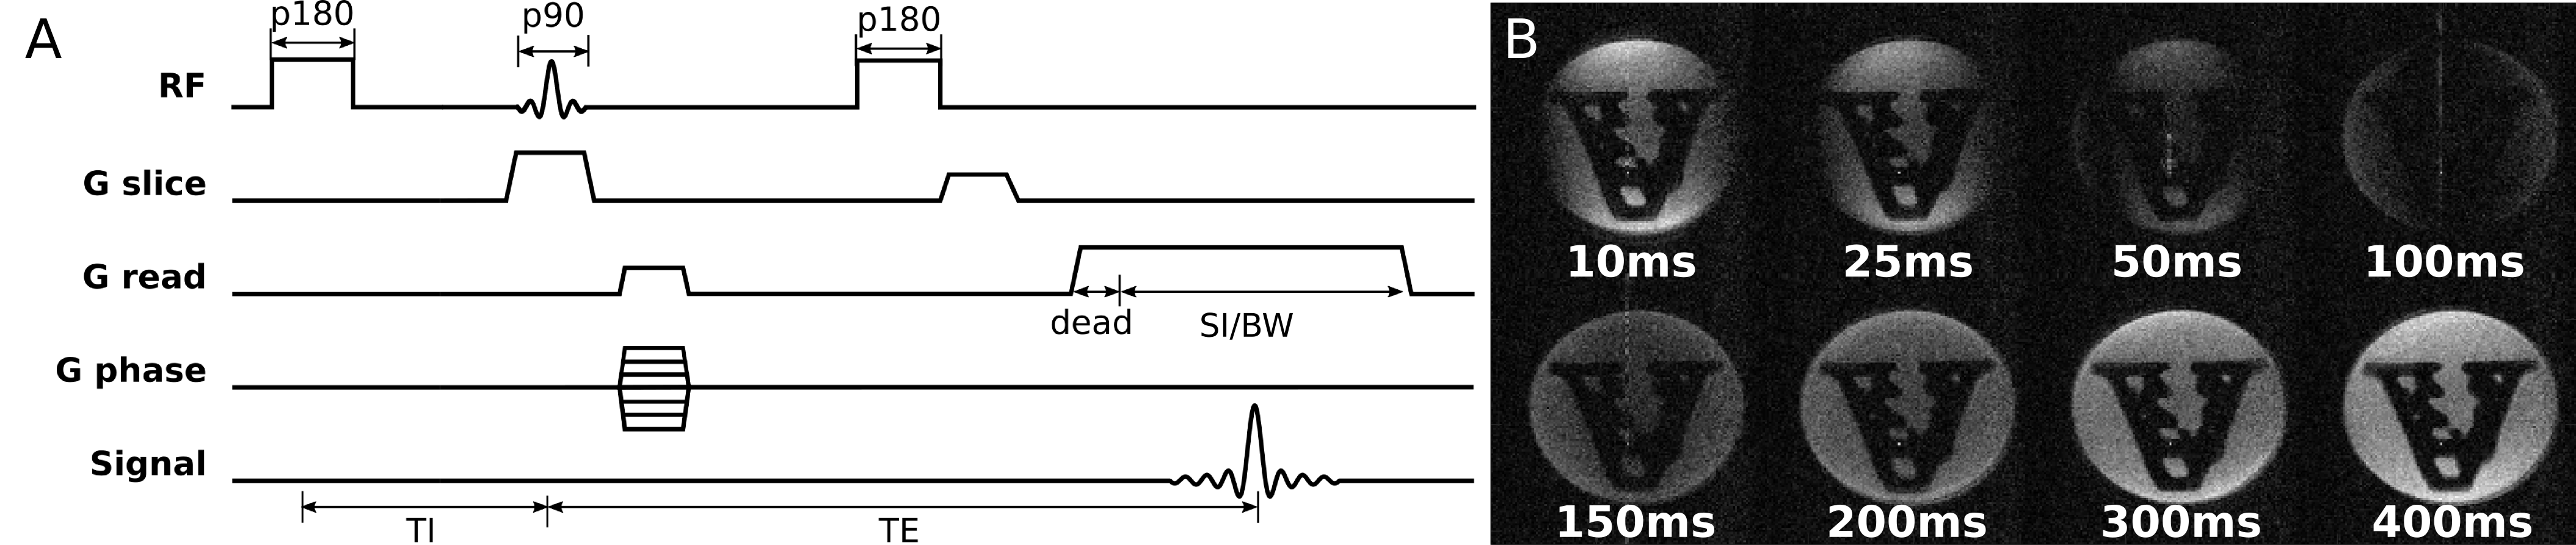
\includegraphics[width = 1\textwidth,trim=0 0 0 0,clip=false]{IR_results.png}
\caption{{(A) Slice-selective inversion recovery spin echo pulse sequence generated by \texttt{invrecov.py}. 
(B) A series of 128$\times$128 images with varying inversion times, acquired with 5 mm slice thickness.}}
\label{fig:ir_image}
\end{center}
\end{figure}

\subsection*{Synchronization Analysis}
Table \ref{table:sync_table} shows how often desynchronization events occurred during the \texttt{spinecho.py} sequence,
with and without running Interactive Mode prior to running the scan.
The Table shows that the described monitoring function corrected the desynchronization event each time by adjusting the leader and follower delays to compensate.
Desynchronization events occur more frequently immediately after starting a flowgraph 
because the USB interface dynamically optimizes the data buffer sizes.
By running interactive mode first for approximately 30 seconds, 
the buffer sizes were more likely to stabilize prior to running the full scan.
In that case, only one desynchronization even occurred, and there were no data corruptions.
When Interactive Mode was not run, 
one of the ten desynchronization events led to data corruption.
Data corruption is the result of a desynchronization event that occurs between the 
most recent check for synchronization and the time at which the pulses are transmitted.

\begin{table}
\begin{tabular}{| c | c | c |}
	\hline
	 & \textbf{Interactive Mode Off} & \textbf{Interactive Mode On} \\ \hline
	\textbf{TR (s)} & 1 & 1 \\ \hline
	\textbf{Scan Time (s)} & 128 & 128 \\ \hline
	\textbf{Scans Run} & 15 & 15 \\ \hline
	\textbf{Desync Detected} & 10 (66\%) & 1 (6.6\%) \\ \hline
	\textbf{Desync Corrected} & 10 (100\%) & 1 (100\%) \\ \hline
	\textbf{Data Corrupted} & 1 (10\%) & 0 (0\%) \\ \hline
\end{tabular}
\caption{Frequency of desynchronization events and recovery from them, 
with and without entering Interactive Mode before starting an imaging scan.}
\label{table:sync_table}
\end{table}

\subsection*{Frequency-Swept Pulse Generation}

\begin{figure}[h]
\begin{center}
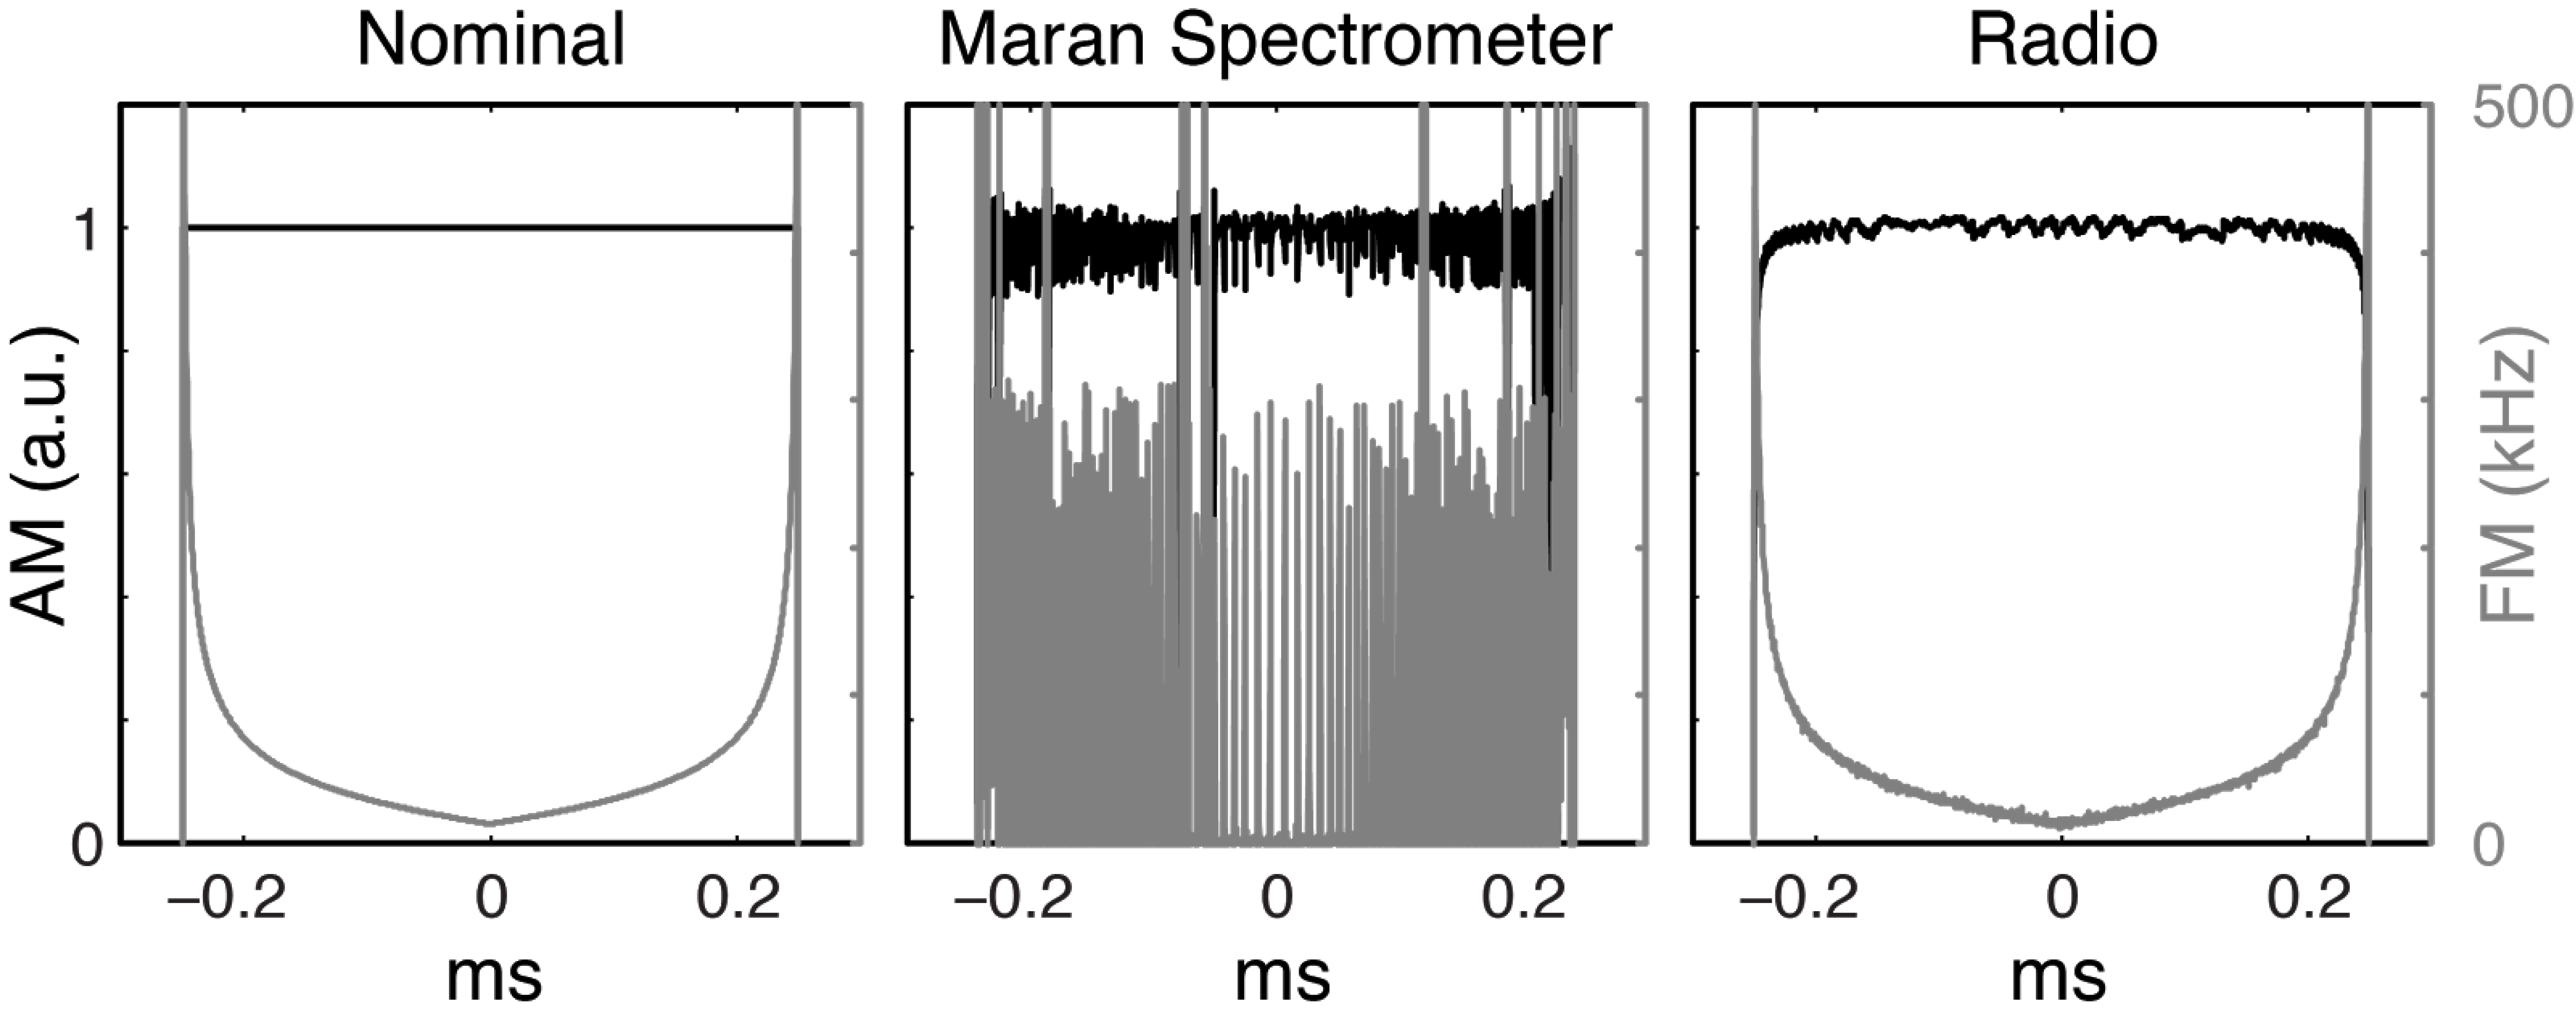
\includegraphics[width = 1\textwidth,trim=0 0 0 0,clip=false]{frequency_sweep.png}
\caption{{Comparison of nominal and measured amplitude modulation (AM) and frequency modulation (FM) waveforms of frequency-swept pulses generated by the Maran spectrometer and the SDR
with the gr-MRI Triggered Vector Source block.}}
\label{fig:f_sweep}
\end{center}
\end{figure}

Figure \ref{fig:f_sweep} compares small-signal frequency-swept pulses generated by the Maran and the USRP1 with gr-MRI. 
The USRP1 played the waveform with high fidelity, 
while the Maran’s waveform contained spurious dropouts and undesired phase plateaus due to limited temporal and phase resolution, 
resulting in large spikes in the transmitted FM waveform.
The RMS error of the Maran's amplitude waveform was 24.8\%, 
while that of the radio's 5.1\%. 
The RMS error of the Maran's frequency waveform was 247 kHz.
The gr-MRI errors were dominated by errors in the first and last samples of the measured waveforms.

\section*{Discussion}
\subsection*{Summary of Results}
We presented the gr-MRI software package, which comprises a set of Python scripts, flowgraphs, and 
signal generation and recording blocks for GNU Radio, 
an open-source SDR software package that is widely used in communications research. 
gr-MRI Implements basic sequencing functionality, 
and tools for system calibrations, multi-radio synchronization, and 
MR signal processing and image reconstruction. 
It includes four pulse sequences: 
a single-pulse sequence to record free induction signals, 
a gradient-recalled echo imaging sequence, a spin echo imaging sequence,
and a spin echo inversion recovery imaging sequence.

\par The imaging sequences were validated in 0.5 T phantom imaging experiments, 
and the gradient-recalled echo and 
spin echo images were compared to images acquired using a commercial MRI spectrometer.
The images were free of distortions and had higher apparent SNR than the Maran images. 
The reason for the SNR difference is unknown; the sequences were carefully matched and the same
coil and amplifiers were used for both. 
Thus we do not wish to draw any conclusions from that SNR difference;
rather, the image comparison to the Maran spectrometer demonstrates geometric fidelity of 
the gr-MRI images.
The ability to generate frequency-swept pulses using gr-MRI was also validated, 
which is needed for adiabatic excitations \cite{Garwood:2001:J-Magn-Reson:11740891}
and may be useful for RF encoding using the Bloch-Siegert shift \cite{kartausch:13,cao:ismrm14}. 

\subsection*{SDR Considerations}
gr-MRI was validated in this work using Ettus Research USRP1's.
The USRP1 is the first Ettus SDR and has a more basic feature set than 
more recent models (though it was available for purchase from Ettus at the time of writing). 
The software is compatible with any GNU Radio-compatible SDR,
though some of the features we developed based on the USRP1's capabilities 
may not be required for newer SDRs.
For example, some newer SDRs have gigabit ethernet connections to the PC,
which reduces latency by a few orders of magnitude compared to USB. 
We used looped-back signals as a general solution to latency and between-radio delays;
with lower and more stable latency, pulse sequences may not require this.
Additionally, some modern SDRs allow for time synchronization via time-stamped transmissions 
or with a MIMO cable.
These simplifications would free up valuable I/O channels.
In addition, 
radios with more channels may be able to perform both RF and gradient functions. 

\par Another consideration is Larmor frequency: 
the USRP1 can directly synthesize signals up to 64 MHz, 
so to operate at higher frequencies the user would need to use high-frequency transmit/receive daughterboards with onboard modulation/demodulation circuits,
or implement mixing externally.
Care would need to be taken to make sure that the reference oscillator signals for modulation
and demodulation are phase-locked.

\par To obtain a 6 V RF amplifier unblanking pulse, 
we used the SDR's 1 V transmit enable pulse to turn on a transistor switch that connected a 6 V DC power source to the amplifier whenever the pulse was high.
It may be possible to use SDR I/O pins to produce these and other control signals (such as signals 
needed for coil detuning circuits); such pins exist on the USRP1 motherboard but 
are not currently supported by GNU Radio. 

\section*{Conclusion}
gr-MRI enables commercially-available software-defined radios
to be used as 
low-cost custom MRI spectrometers, with fidelity that is comparable to or better than
commercial spectrometers.
It was designed to be highly customizable and reconfigurable. 
This will make it easier for researchers and engineers to develop custom spectrometers, 
without requiring significant spectrometer hardware development
or FPGA programming.

\section*{Acknowledgments}

This work was supported by NIH R21 EB 018521.


%\nolinenumbers

\bibliography{gr_MRI}{}
\bibliographystyle{plos2015}


\end{document}

